% !TEX program = xelatex
\documentclass[12pt,a4paper]{article}

% ===== 中文支持 =====
\usepackage{xeCJK}
\setCJKmainfont{SimSun}[BoldFont=SimHei,ItalicFont=KaiTi]
\setCJKsansfont{SimHei}
\setCJKmonofont{FangSong}
\xeCJKsetup{PunctStyle=banjiao}

% ===== 页面设置 =====
\usepackage[top=2.5cm,bottom=2.5cm,left=2.5cm,right=2.5cm]{geometry}

% ===== 常用宏包 =====
\usepackage{amsmath,amssymb}
\usepackage{graphicx}
\usepackage{booktabs}
\usepackage{array}
\usepackage{multirow}
\usepackage{longtable}
\usepackage{tabularx}
\usepackage{enumitem}
\usepackage{caption}
\usepackage{subcaption}
\usepackage{float}
\usepackage{listings}
\usepackage{xcolor}
\usepackage{hyperref}
\usepackage{fancyhdr}
\usepackage{titlesec}
\usepackage{setspace}

% ===== 代码样式 =====
\lstdefinestyle{sqlstyle}{
  language=SQL,
  basicstyle=\ttfamily\small,
  keywordstyle=\color{blue}\bfseries,
  stringstyle=\color{red},
  commentstyle=\color{green!60!black}\itshape,
  numbers=left,
  numberstyle=\tiny\color{gray},
  frame=single,
  breaklines=true,
  tabsize=4,
  showstringspaces=false
}
\lstdefinestyle{pythonstyle}{
  language=Python,
  basicstyle=\ttfamily\small,
  keywordstyle=\color{blue}\bfseries,
  stringstyle=\color{red},
  commentstyle=\color{green!60!black}\itshape,
  numbers=left,
  numberstyle=\tiny\color{gray},
  frame=single,
  breaklines=true,
  tabsize=4,
  showstringspaces=false
}

% ===== 超链接设置 =====
\hypersetup{
  colorlinks=true,
  linkcolor=black,
  urlcolor=blue,
  bookmarks=true,
  pdfauthor={严浩睿，马沛霖},
  pdftitle={OpenGauss 数据库应用开发 — 企业员工管理系统}
}

% ===== 页眉页脚 =====
\pagestyle{fancy}
\fancyhf{}
\fancyhead[L]{\small 数据库系统 Project 报告}
\fancyhead[R]{\small OpenGauss 企业员工管理系统}
\fancyfoot[C]{\thepage}
\renewcommand{\headrulewidth}{0.4pt}

% ===== 行距 =====
\setstretch{1.5}

% ===== 标题格式 =====
\titleformat{\section}{\Large\bfseries\CJKfamily{SimHei}}{\thesection}{1em}{}
\titleformat{\subsection}{\large\bfseries\CJKfamily{SimHei}}{\thesubsection}{1em}{}
\titleformat{\subsubsection}{\normalsize\bfseries\CJKfamily{SimHei}}{\thesubsubsection}{1em}{}

\begin{document}

% ============================================================
% 目录
% ============================================================
\tableofcontents

% ============================================================
% 小组分工
% ============================================================
\section*{小组分工}
\addcontentsline{toc}{section}{小组分工}

本项目由两名成员合作完成，具体分工如下表所示。在项目开发过程中，两位成员密切配合，定期进行进度同步和技术讨论，确保项目按时高质量完成。

\begin{table}[htbp]
  \centering
  \caption{小组成员及分工}
  \renewcommand{\arraystretch}{1.5}
  \begin{tabular}{cl>{\raggedright\arraybackslash}p{7cm}}
    \toprule
    \textbf{学号} & \textbf{姓名} & \textbf{负责内容} \\
    \midrule
    20240395 & 严浩睿 & 需求分析、E-R 图设计、关系模型设计、数据库建表与优化 \\
    20240640 & 马沛霖 & 数据库物理设计、程序编码实现、数据库连接与 CRUD 操作 \\
    \bottomrule
  \end{tabular}
\end{table}

\textbf{协作说明：} 严浩睿同学主要负责系统前期的需求调研和数据库设计工作，包括业务流程分析、E-R 模型构建、关系模式转换及数据库表结构设计。马沛霖同学主要负责数据库的物理实现和应用程序开发，包括 OpenGauss 数据库部署、SQL 语句编写、Python 程序开发及系统测试。两位同学在项目关键节点进行了充分的技术交流和方案讨论。

% ============================================================
% 第 1 章 背景分析
% ============================================================
\section{企业员工管理系统背景分析}

\subsection{项目背景}

随着企业规模的不断扩大和信息化建设的深入推进，传统的纸质档案管理和人工统计方式已无法满足现代企业对员工信息管理的需求。企业员工信息涉及个人基本信息、部门、岗位、薪资、考勤等多个维度，数据量大且更新频繁，亟需一套高效、可靠的管理系统来实现对员工信息的集中管理和快速查询。

从行业发展角度来看，人力资源管理信息化已成为企业数字化转型的重要组成部分。根据相关调研数据显示，超过 80\% 的中大型企业已采用或计划采用电子化的人力资源管理系统。这些系统不仅能够提高人事部门的工作效率，还能为管理层提供数据支持，辅助决策制定。

本系统基于国产数据库 OpenGauss，设计并实现一个小型的企业员工管理系统。OpenGauss 是由华为开源的企业级关系型数据库，具有高性能、高可用、高安全等特点，适用于各类企业应用场景。选择 OpenGauss 作为本系统的数据库平台，主要基于以下考虑：

\begin{enumerate}[label=(\arabic*)]
  \item \textbf{技术先进性：} OpenGauss 基于 PostgreSQL 发展而来，支持丰富的数据类型和先进的查询优化技术；
  \item \textbf{自主可控：} 作为国产开源数据库，OpenGauss 在信息安全方面具有优势，符合国家信创战略要求；
  \item \textbf{生态完善：} OpenGauss 提供了完善的开发工具和管理平台，便于系统开发和维护；
  \item \textbf{性能优异：} 针对企业级应用场景进行了深度优化，能够支持高并发和大容量数据处理。
\end{enumerate}

\subsection{系统目标}

本系统旨在实现以下目标：

\begin{enumerate}[label=(\arabic*)]
  \item \textbf{数据集中管理：} 建立规范化的企业员工信息数据库，实现员工信息的统一存储和管理，避免数据分散和重复；
  \item \textbf{功能完善：} 提供完善的数据增删改查（CRUD）功能，满足日常员工信息管理需求，包括员工入职、调岗、离职等全生命周期管理；
  \item \textbf{数据质量保障：} 确保数据的一致性和完整性，通过主键、外键、检查约束等数据库机制减少数据冗余和异常；
  \item \textbf{易用性：} 提供友好的用户交互界面，降低使用门槛，使非技术人员也能轻松操作系统；
  \item \textbf{可扩展性：} 系统架构设计考虑未来功能扩展需求，便于后续添加绩效考核、培训管理等模块。
\end{enumerate}

\subsection{需求分析}

通过对企业员工管理业务的深入分析，本系统需要管理以下核心信息：

\begin{itemize}
  \item \textbf{员工信息管理：} 员工的基本信息（姓名、性别、出生日期、联系方式、入职日期等）的录入、修改、删除和查询。需要支持按部门、岗位、入职时间等多条件筛选。
  \item \textbf{部门信息管理：} 部门的创建、修改、删除和查询，以及部门与员工之间的归属关系。需要统计各部门人员数量，支持组织架构图展示。
  \item \textbf{岗位信息管理：} 岗位的设置、调整和查询，以及岗位与员工的对应关系。需要管理岗位职责描述和薪资等级。
  \item \textbf{薪资信息管理：} 员工薪资的录入、调整和查询，包括基本工资、绩效、奖金等。需要支持按月查询和统计报表生成。
  \item \textbf{考勤信息管理：} 员工出勤记录的录入、统计和查询。需要支持正常、迟到、早退、请假、缺勤等多种状态记录。
\end{itemize}

\begin{figure}[htbp]
  \centering
  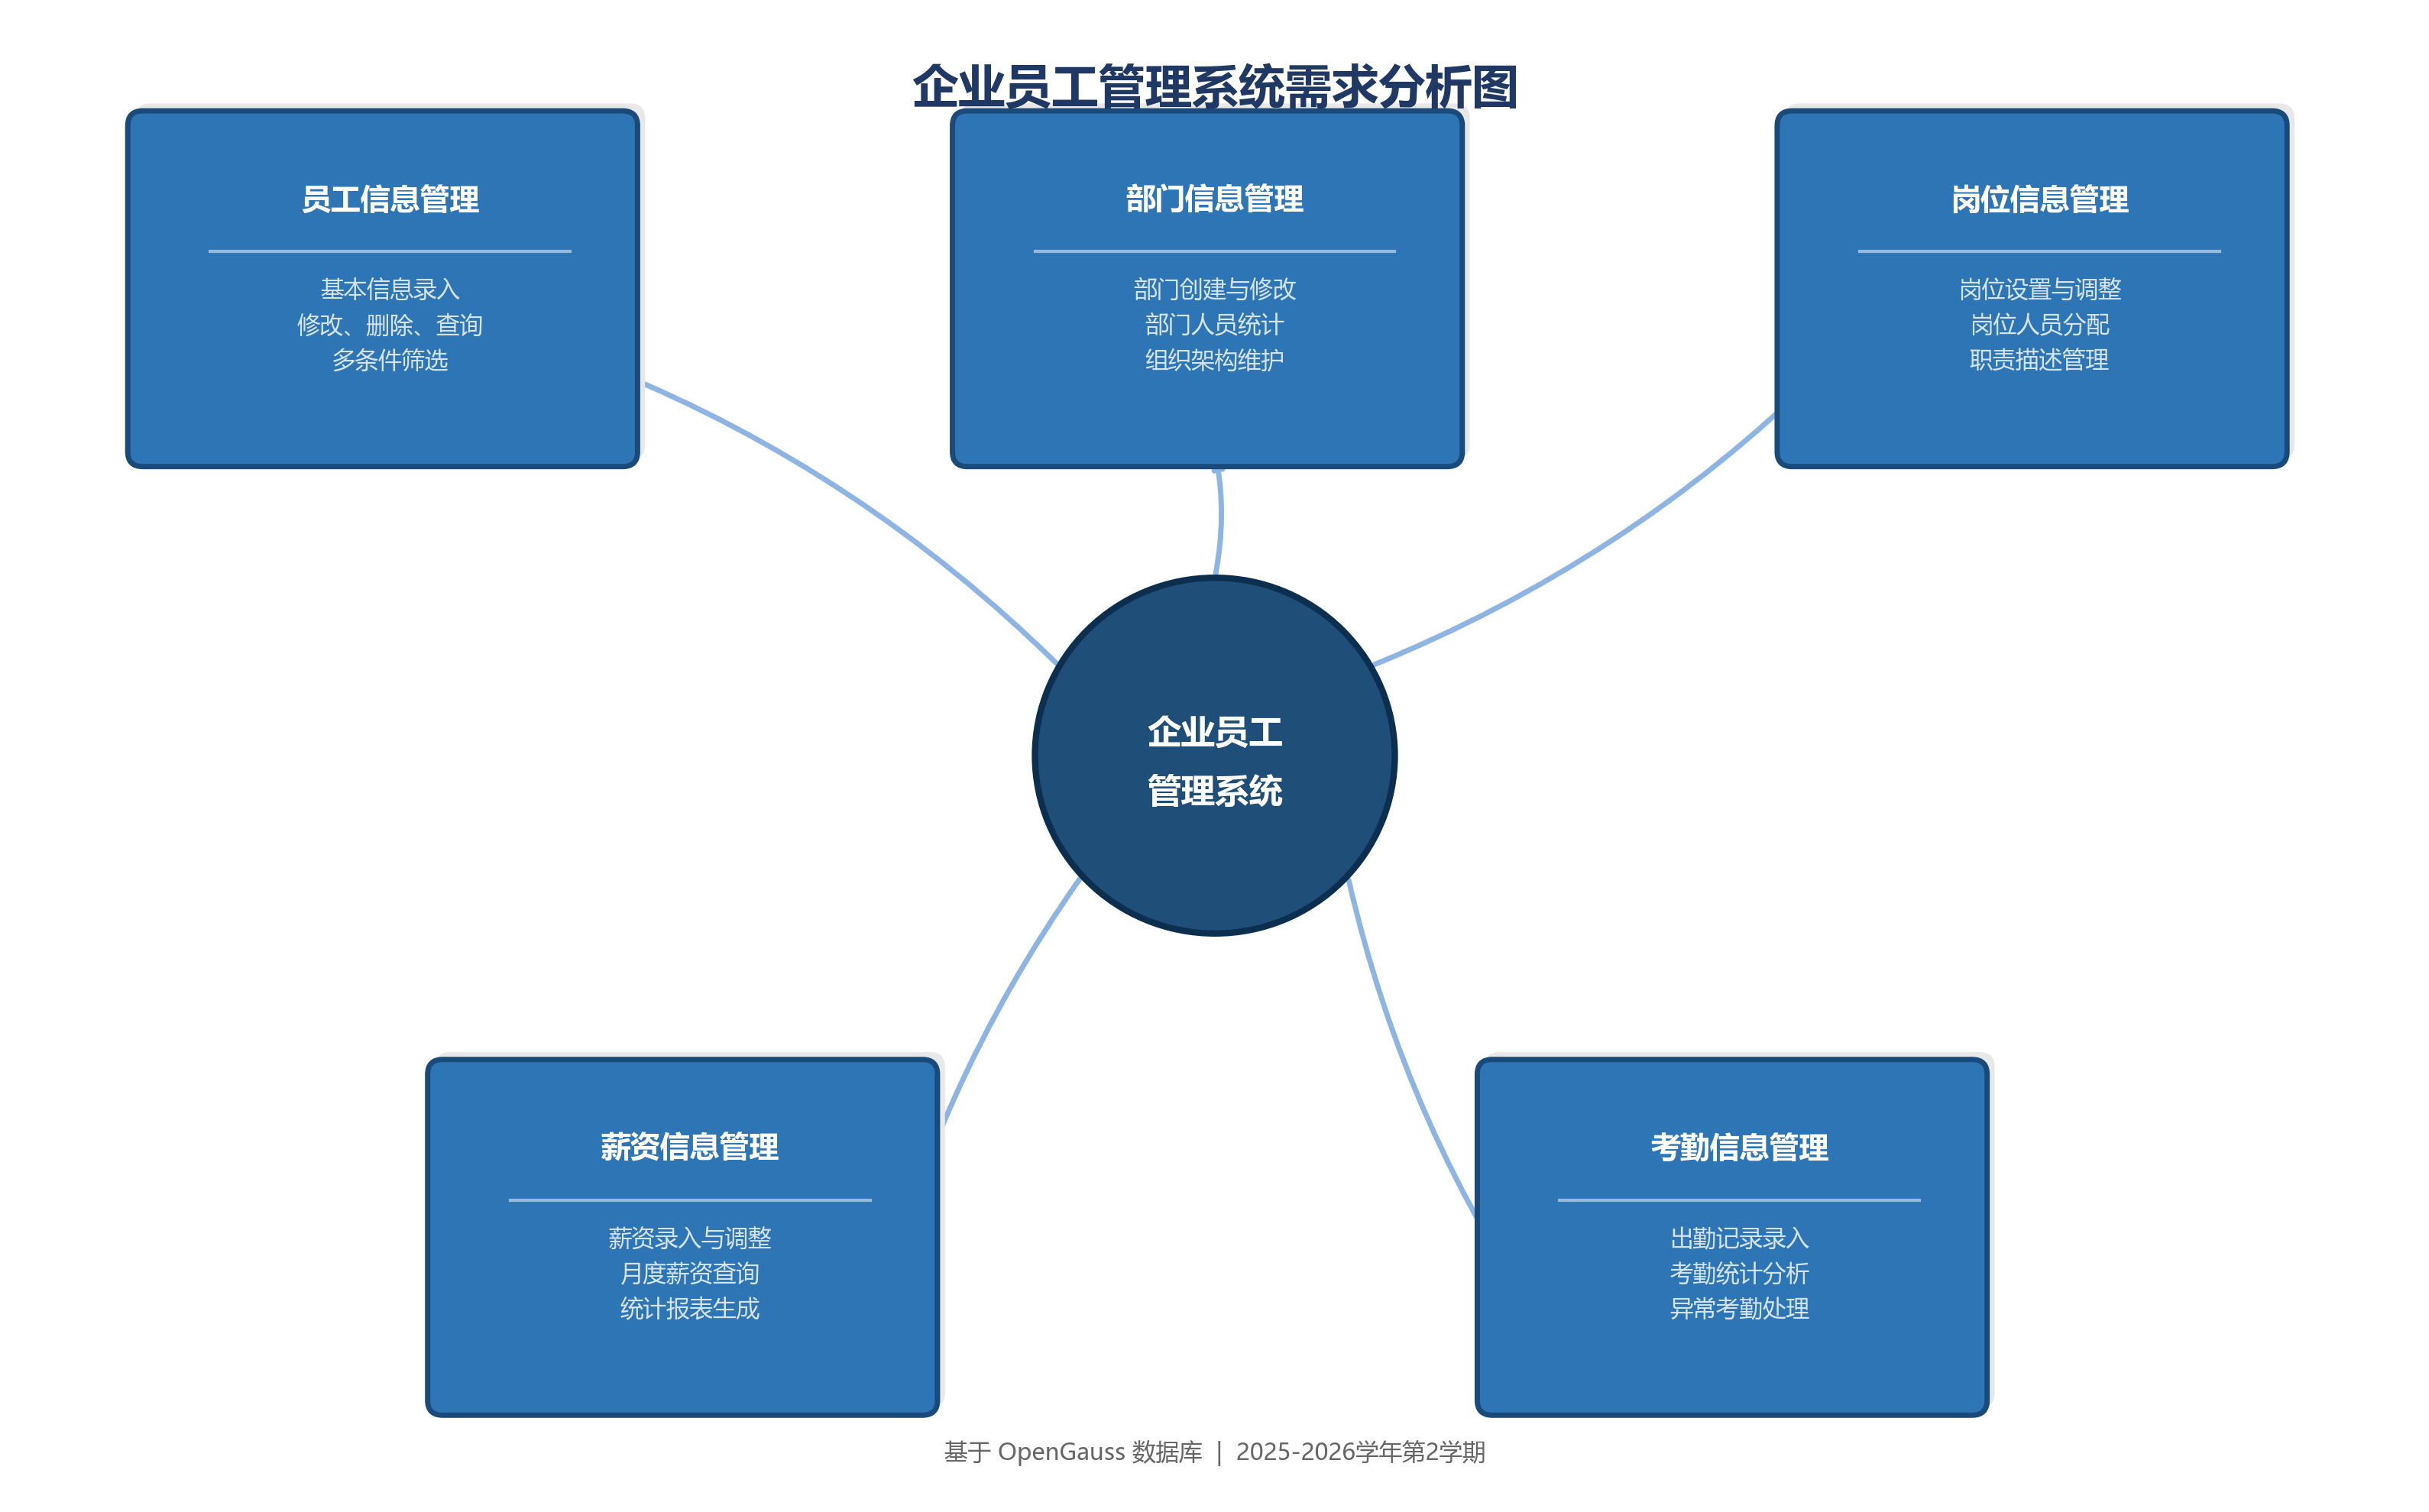
\includegraphics[width=0.95\textwidth]{req_analysis.png}
  \caption{企业员工管理系统需求分析图}
  \label{fig:req-analysis}
\end{figure}

图\ref{fig:req-analysis}展示了系统的五大核心需求模块及其功能要点。每个模块都围绕员工管理的特定业务场景设计，模块之间通过员工实体相互关联，形成完整的业务闭环。

\subsection{系统功能模块设计}

基于上述需求分析，本系统划分为以下功能模块：

\begin{table}[htbp]
  \centering
  \caption{系统功能模块}
  \renewcommand{\arraystretch}{1.4}
  \begin{tabularx}{\textwidth}{>{\centering\arraybackslash}p{1.5cm} >{\raggedright\arraybackslash}p{2.5cm} >{\raggedright\arraybackslash}X}
    \toprule
    \textbf{模块编号} & \textbf{模块名称} & \textbf{功能描述} \\
    \midrule
    M1 & 员工管理模块 & 员工信息的增删改查，支持多条件筛选，员工档案管理 \\
    M2 & 部门管理模块 & 部门信息的增删改查，部门人员统计，组织架构维护 \\
    M3 & 岗位管理模块 & 岗位信息的增删改查，岗位人员分配，职责描述管理 \\
    M4 & 薪资管理模块 & 薪资信息的录入、调整和查询统计，薪资报表生成 \\
    M5 & 考勤管理模块 & 考勤记录的录入、统计和报表生成，异常考勤处理 \\
    \bottomrule
  \end{tabularx}
\end{table}

各模块之间的业务关系如下：员工管理模块是系统的核心，与其他所有模块都存在数据关联。部门管理模块和岗位管理模块为员工管理提供基础数据支持。薪资管理模块和考勤管理模块则基于员工信息进行业务数据记录和分析。

\begin{figure}[htbp]
  \centering
  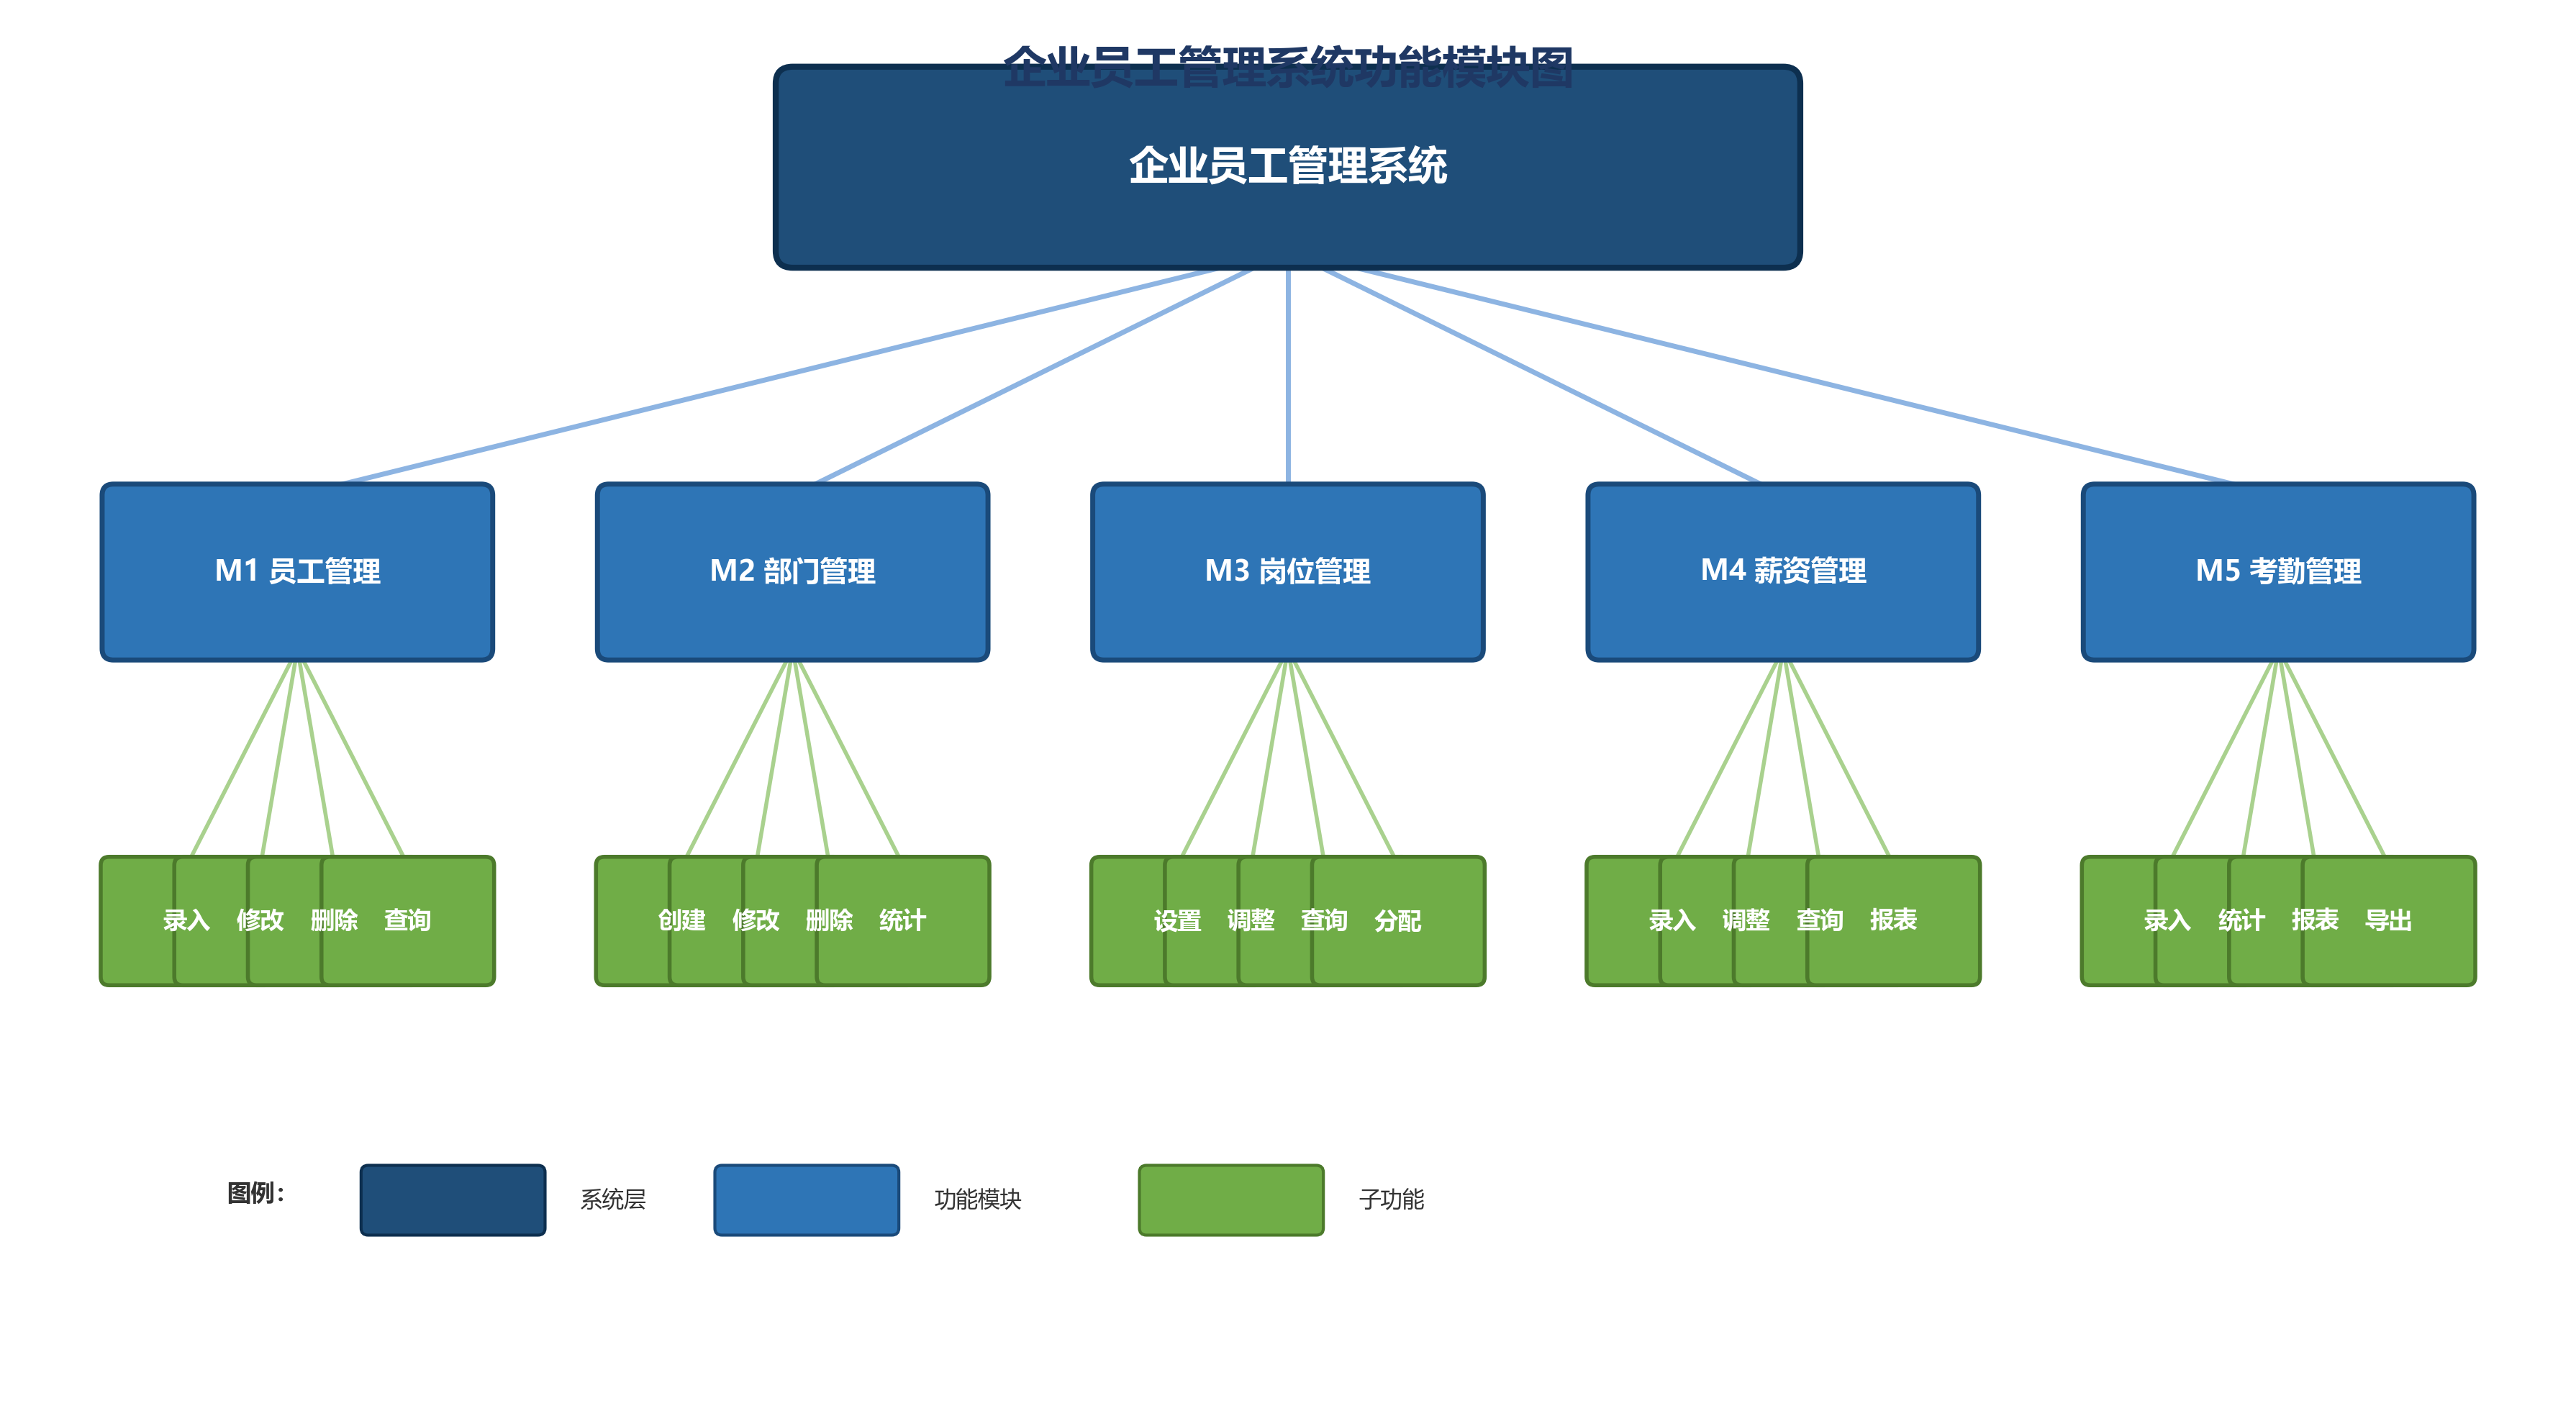
\includegraphics[width=0.95\textwidth]{func_modules.png}
  \caption{企业员工管理系统功能模块图}
  \label{fig:func-modules}
\end{figure}

图\ref{fig:func-modules}以树状结构展示了系统的功能模块层次关系。系统层包含五个一级功能模块，每个一级模块下又细分为若干子功能，形成了清晰的功能架构。

% ============================================================
% 第 2 章 概念设计
% ============================================================
\section{企业员工管理系统概念设计}

\subsection{实体识别}

通过对系统需求的分析，识别出以下核心实体：

\begin{enumerate}
  \item \textbf{员工（Employee）：} 系统中的核心实体，记录每位员工的个人信息。员工是企业的基本组成单位，所有其他业务数据都围绕员工展开。
  \item \item \textbf{部门（Department）：} 企业的组织单位，与员工存在归属关系。部门反映了企业的组织架构，是员工管理的重要维度。
  \item \textbf{岗位（Position）：} 员工的职务岗位，与员工存在对应关系。岗位决定了员工的职责范围和薪资等级。
  \item \textbf{薪资（Salary）：} 员工的薪资记录，与员工存在关联。薪资是员工报酬的量化体现，需要按月记录和管理。
  \item \textbf{考勤（Attendance）：} 员工的出勤记录，与员工存在关联。考勤反映了员工的工作状态，是薪资计算的重要依据。
\end{enumerate}

\subsection{实体属性}

各实体的主要属性如下表所示：

\begin{table}[htbp]
  \centering
  \caption{实体及其属性}
  \renewcommand{\arraystretch}{1.4}
  \begin{tabularx}{\textwidth}{>{\raggedright\arraybackslash}p{1.8cm} >{\raggedright\arraybackslash}p{2cm} >{\raggedright\arraybackslash}X}
    \toprule
    \textbf{实体} & \textbf{主键} & \textbf{主要属性} \\
    \midrule
    员工 & emp\_id & 姓名、性别、出生日期、电话、邮箱、入职日期 \\
    部门 & dept\_id & 部门名称、部门描述、负责人 \\
    岗位 & pos\_id & 岗位名称、岗位描述、薪资等级 \\
    薪资 & salary\_id & 基本工资、绩效工资、奖金、发放月份 \\
    考勤 & attend\_id & 考勤日期、出勤状态、备注 \\
    \bottomrule
  \end{tabularx}
\end{table}

\textbf{属性设计说明：}
\begin{itemize}
  \item 所有实体都采用自增整数作为主键，确保记录的唯一性和查询效率；
  \item 员工实体的邮箱属性设置为 UNIQUE 约束，保证邮箱地址不重复；
  \item 性别属性采用单字符存储（M/F），节省存储空间；
  \item 薪资和考勤实体通过外键关联到员工实体，建立数据关联关系。
\end{itemize}

\subsection{实体间联系}

\begin{itemize}
  \item \textbf{部门---员工：} 1 对多联系。一个部门可以有多名员工，一名员工属于一个部门。这种联系反映了企业的组织架构，通过 Employee 表中的 dept\_id 外键实现。
  \item \textbf{岗位---员工：} 1 对多联系。一个岗位可以有多名员工，一名员工担任一个岗位。这种联系体现了岗位与人员的对应关系，通过 Employee 表中的 pos\_id 外键实现。
  \item \textbf{员工---薪资：} 1 对多联系。一名员工可以有多条薪资记录（按月发放）。这种联系支持薪资的历史查询和趋势分析。
  \item \textbf{员工---考勤：} 1 对多联系。一名员工可以有多条考勤记录（按日记录）。这种联系支持考勤的詳細统计和报表生成。
\end{itemize}

\subsection{E-R 图}

根据以上分析，绘制出系统的 E-R 图如图\ref{fig:er}所示。

\begin{figure}[htbp]
  \centering
  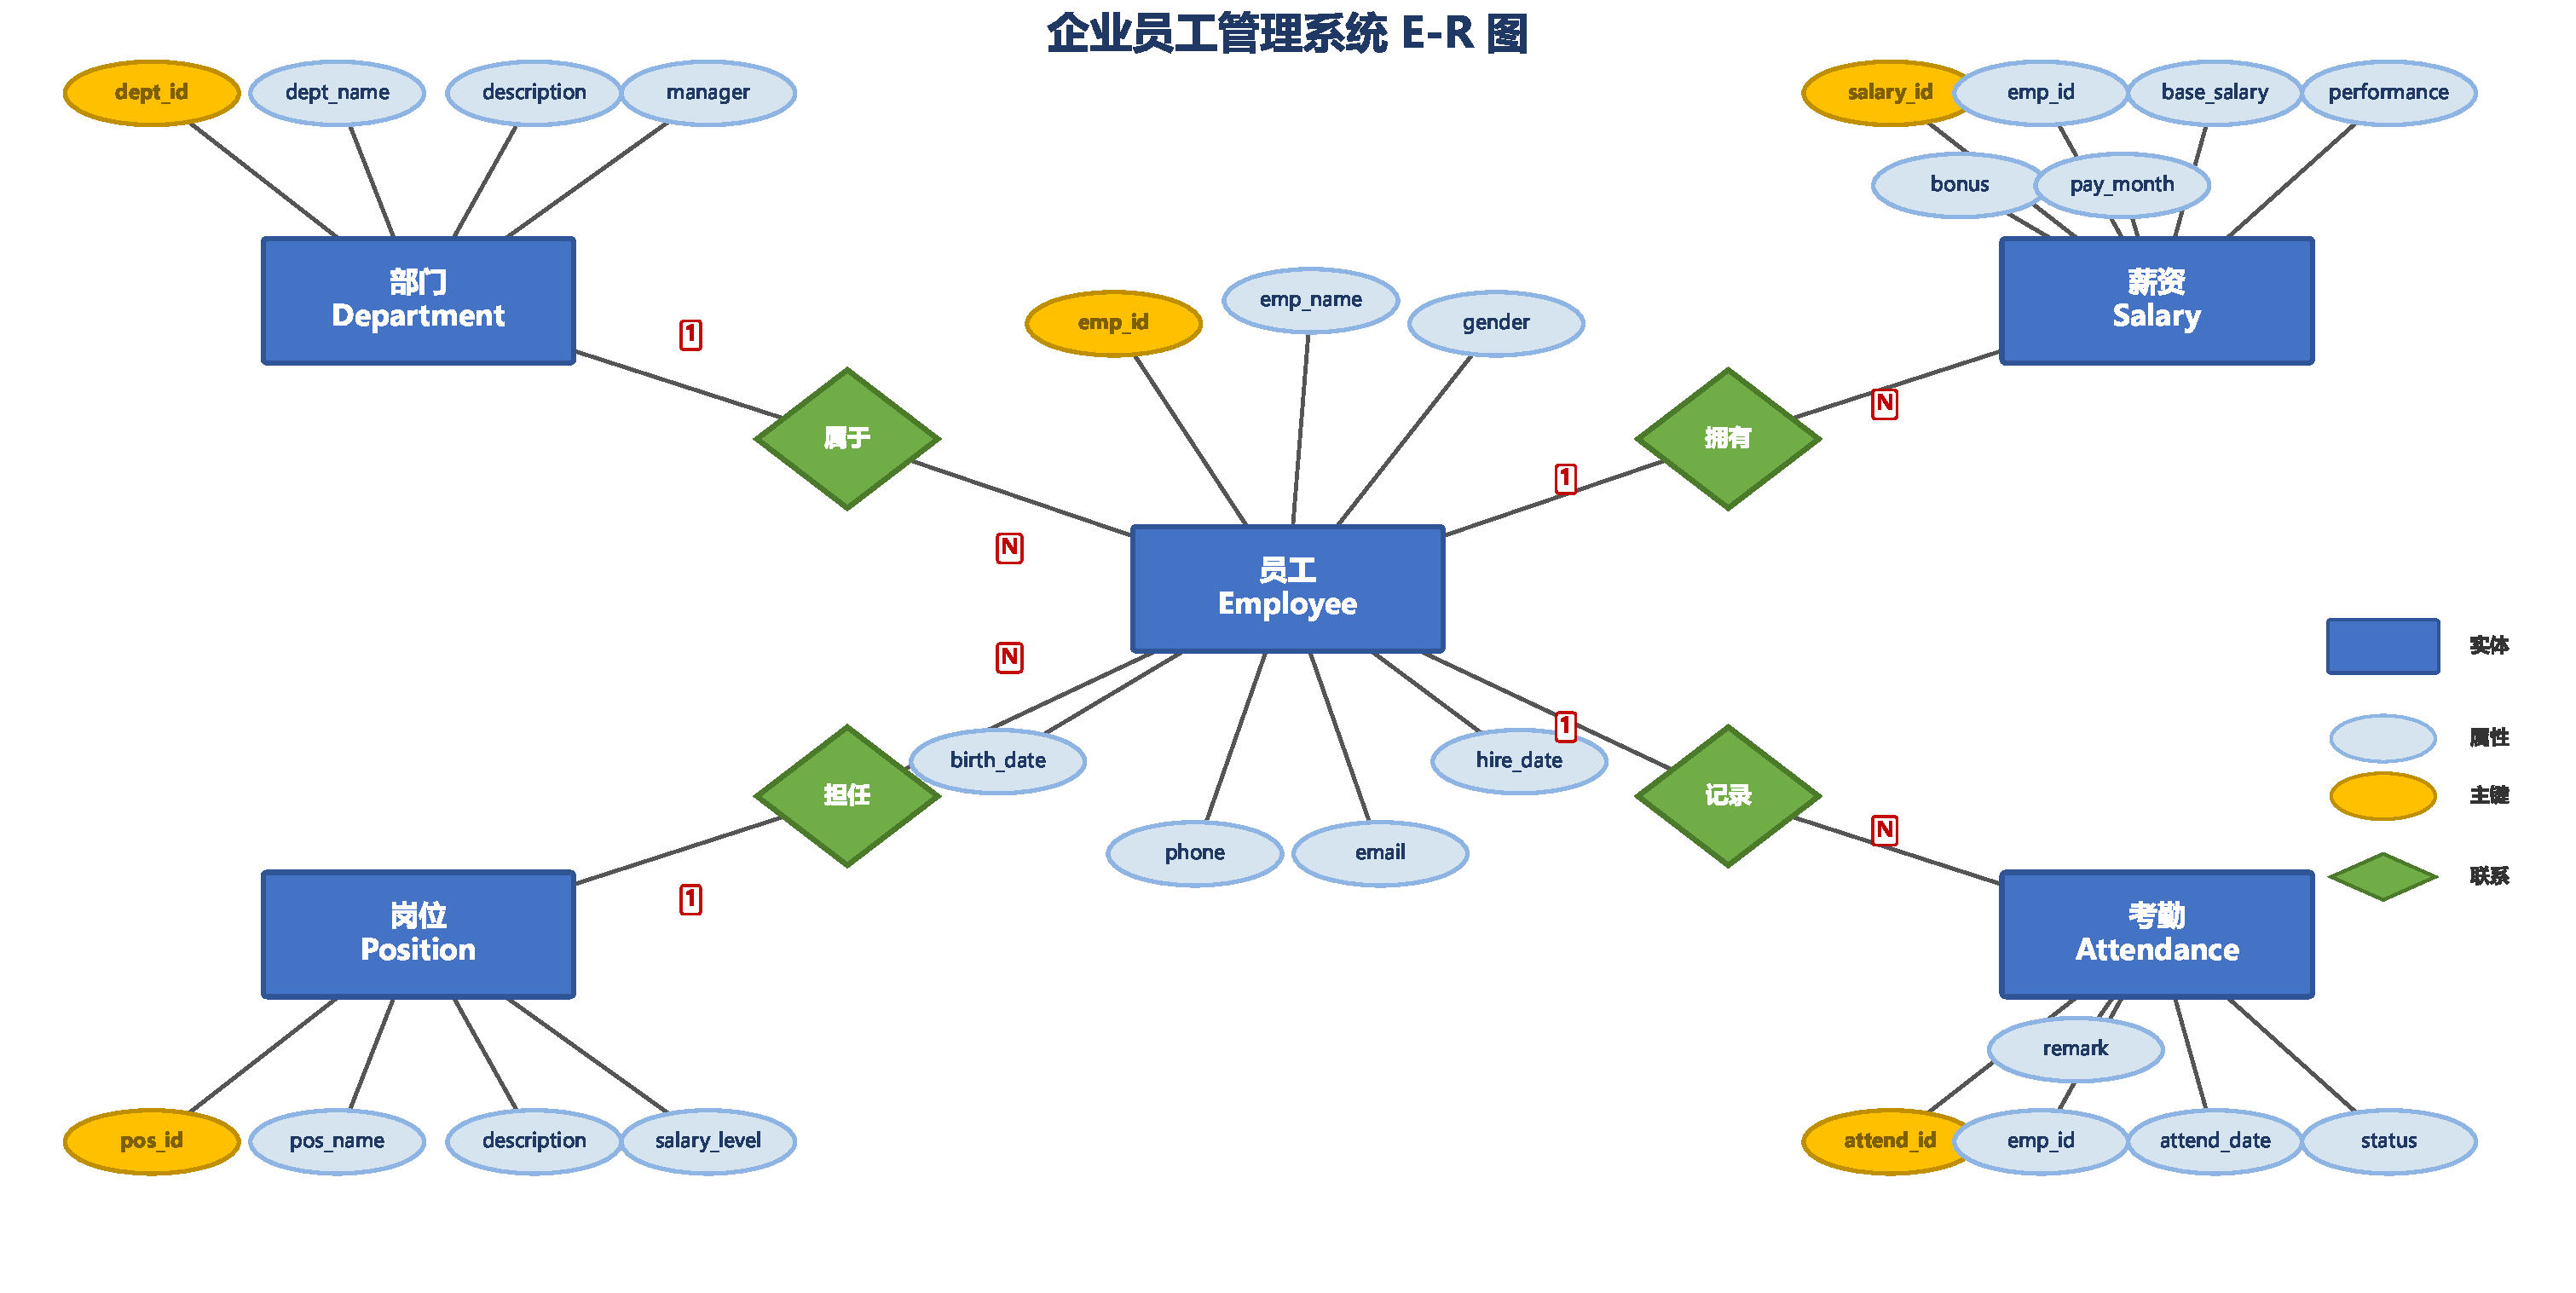
\includegraphics[width=0.95\textwidth]{er_diagram.pdf}
  \caption{企业员工管理系统 E-R 图}
  \label{fig:er}
\end{figure}

\textbf{E-R 图说明：}
\begin{itemize}
  \item \textbf{矩形}（蓝色）表示实体：员工、部门、岗位、薪资、考勤；
  \item \textbf{椭圆}（浅蓝）表示属性，\textbf{金色椭圆}（带下划线）表示主键属性；
  \item \textbf{菱形}（绿色）表示联系：属于、担任、拥有、记录；
  \item 连线上的数字（\textcolor{red}{1}、\textcolor{red}{N}）表示联系的基数，均为一对多（1:N）联系。
\end{itemize}

\textbf{联系详解：}
\begin{itemize}
  \item 部门\,--1--\,属于\,--N--\,员工：一个部门有多名员工，一名员工属于一个部门；
  \item 岗位\,--1--\,担任\,--N--\,员工：一个岗位有多名员工，一名员工担任一个岗位；
  \item 员工\,--1--\,拥有\,--N--\,薪资：一名员工按月有多条薪资记录；
  \item 员工\,--1--\,记录\,--N--\,考勤：一名员工按日有多条考勤记录。
\end{itemize}

% ============================================================
% 第 3 章 关系模型及优化
% ============================================================
\section{企业员工管理系统的关系模型及优化}

\subsection{E-R 图向关系模型的转换}

根据 E-R 图，将实体和联系转换为以下关系模式：

\begin{enumerate}
  \item \textbf{Department}(\underline{dept\_id}, dept\_name, description, manager)
  \item \textbf{Position}(\underline{pos\_id}, pos\_name, description, salary\_level)
  \item \textbf{Employee}(\underline{emp\_id}, emp\_name, gender, birth\_date, phone, email, hire\_date, \textit{dept\_id}, \textit{pos\_id})
  \item \textbf{Salary}(\underline{salary\_id}, \textit{emp\_id}, base\_salary, perf\_bonus, bonus, pay\_month)
  \item \textbf{Attendance}(\underline{attend\_id}, \textit{emp\_id}, attend\_date, status, remark)
\end{enumerate}

其中，下划线表示主键，斜体表示外键。

\textbf{转换规则说明：}
\begin{itemize}
  \item 每个实体转换为一个关系模式，实体的属性即为关系的属性；
  \item 实体的主键转换为关系的主键；
  \item 1:N 联系通过在外键端（N 端）添加外键属性实现，外键引用 1 端的主键；
  \item 所有联系都转换为外键约束，确保引用完整性。
\end{itemize}

\subsection{关系模型优化}

对上述关系模型进行规范化分析：

\textbf{1NF 分析：} 所有关系的每个属性都是不可再分的原子值，满足第一范式。例如，员工姓名是一个完整的字符串，没有进一步分解的必要；地址信息虽然可以分解为省、市、区等，但本系统不需要如此详细的地址管理，因此保持原子性即可。

\textbf{2NF 分析：} 各关系模式中的非主属性都完全依赖于主键，不存在部分函数依赖，满足第二范式。以 Employee 关系为例，所有非主属性（emp\_name、gender 等）都完全依赖于主键 emp\_id，不存在只依赖于主键某一部分的情况。

\textbf{3NF 分析：} 各关系模式中不存在非主属性对主键的传递依赖，满足第三范式。例如，Department 关系中的 manager 属性直接依赖于 dept\_id，不存在通过其他属性间接依赖的情况。

\textbf{优化措施：}
\begin{itemize}
  \item \textbf{消除冗余：} 将部门负责人的信息从 Department 表中独立，通过 Employee 表的 dept\_id 外键关联来体现，避免了数据冗余。
  \item \textbf{明确联系：} 在 Employee 表中设置 dept\_id 和 pos\_id 外键，明确了部门与员工的 1:N 联系和岗位与员工的 1:N 联系，减少了冗余数据。
  \item \textbf{保证完整性：} 薪资表和考勤表通过 emp\_id 外键关联到员工表，保证了数据的一致性和引用完整性。
  \item \textbf{索引优化：} 为常用查询字段创建索引，提高查询效率。
\end{itemize}

\begin{figure}[htbp]
  \centering
  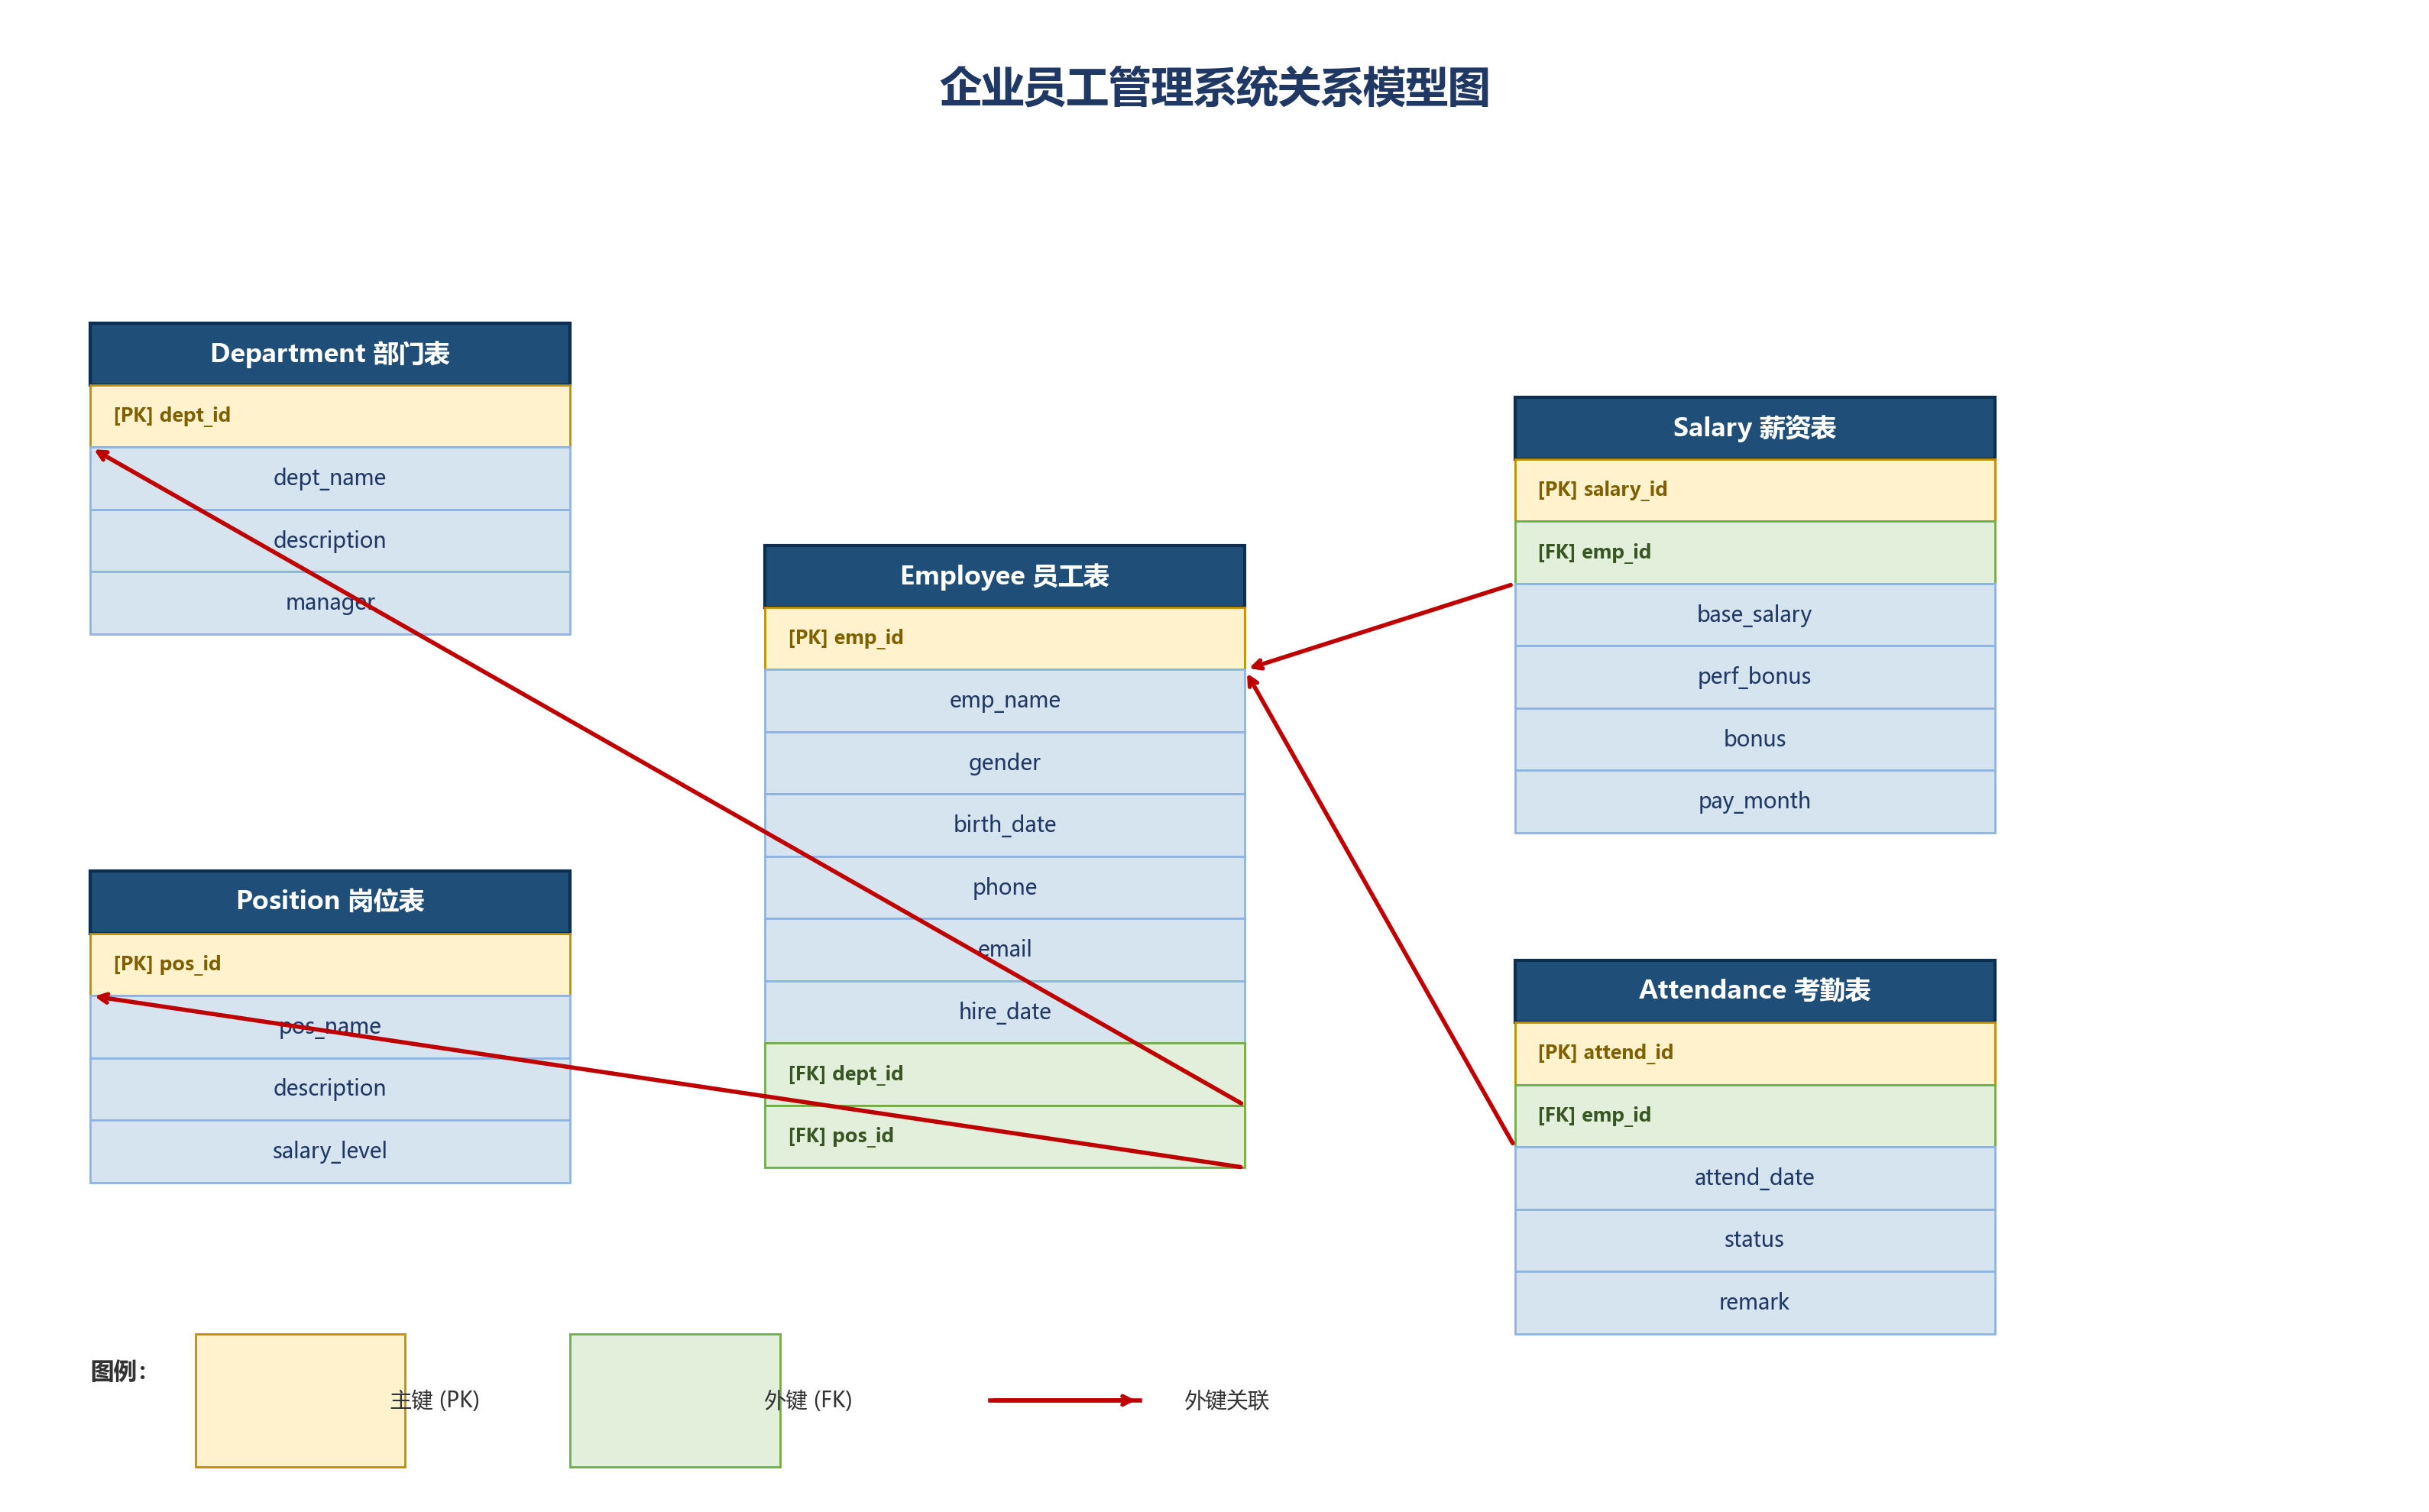
\includegraphics[width=0.95\textwidth]{rel_model.png}
  \caption{企业员工管理系统关系模型图（PK=主键，FK=外键，红色箭头=外键关联）}
  \label{fig:rel-model}
\end{figure}

图\ref{fig:rel-model}展示了系统的完整关系模型，包括五个关系模式的结构和它们之间的外键关联关系。图中用不同颜色区分了主键（金色）和外键（绿色），红色箭头表示外键引用方向。

% ============================================================
% 第 4 章 数据库物理设计
% ============================================================
\section{企业员工管理系统数据库物理设计}

\subsection{数据库创建}

在 OpenGauss 数据库中创建企业员工管理系统的数据库，SQL 语句如下：

\begin{lstlisting}[style=sqlstyle, caption={创建数据库}]
-- 创建数据库
CREATE DATABASE employee_db;
\end{lstlisting}

\begin{figure}[htbp]
  \centering
  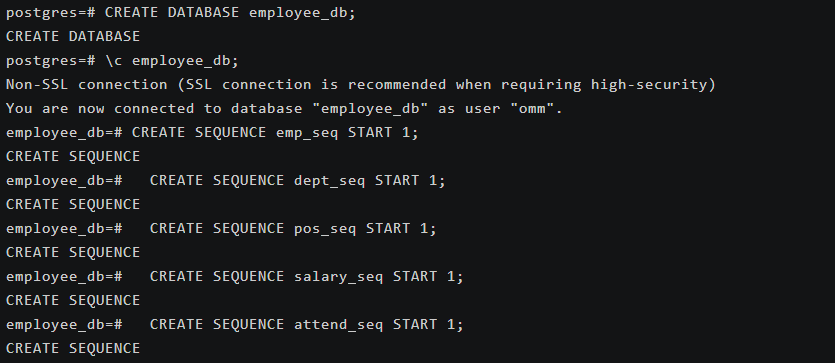
\includegraphics[width=0.9\textwidth]{7a0127c92044cc458ce08a89e9f12a7e.png}
  \caption{创建数据库 employee\_db 及序列}
  \label{fig:create-db}
\end{figure}

图\ref{fig:create-db}展示了在 OpenGauss 中创建数据库和序列的执行过程。序列（Sequence）用于自动生成主键值，确保每条记录的唯一性。本系统为每个表都创建了对应的序列，如 emp\_seq、dept\_seq 等。

\subsection{数据表设计}

根据关系模型，设计以下数据表：

\subsubsection{部门表（Department）}

\begin{table}[htbp]
  \centering
  \caption{Department 表结构}
  \renewcommand{\arraystretch}{1.3}
  \begin{tabularx}{\textwidth}{l l l X}
    \toprule
    \textbf{字段名} & \textbf{数据类型} & \textbf{约束} & \textbf{说明} \\
    \midrule
    dept\_id & INT & PRIMARY KEY & 部门编号，主键，自增 \\
    dept\_name & VARCHAR(50) & NOT NULL & 部门名称，不允许为空 \\
    description & VARCHAR(200) & & 部门描述，可选 \\
    manager & VARCHAR(50) & & 部门负责人，可选 \\
    \bottomrule
  \end{tabularx}
\end{table}

\textbf{设计说明：} 部门表是系统的基础数据表之一，存储企业的组织架构信息。dept\_name 设置为 NOT NULL 约束，确保每个部门都有名称。description 和 manager 字段允许为空，因为新创建的部门可能暂时没有详细描述或负责人。

\subsubsection{岗位表（Position）}

\begin{table}[htbp]
  \centering
  \caption{Position 表结构}
  \renewcommand{\arraystretch}{1.3}
  \begin{tabularx}{\textwidth}{l l l X}
    \toprule
    \textbf{字段名} & \textbf{数据类型} & \textbf{约束} & \textbf{说明} \\
    \midrule
    pos\_id & INT & PRIMARY KEY & 岗位编号，主键，自增 \\
    pos\_name & VARCHAR(50) & NOT NULL & 岗位名称，不允许为空 \\
    description & VARCHAR(200) & & 岗位描述，可选 \\
    salary\_level & INT & & 薪资等级，1-10 级 \\
    \bottomrule
  \end{tabularx}
\end{table}

\textbf{设计说明：} 岗位表管理企业的职位体系。salary\_level 字段用于关联薪资标准，便于后续薪资计算和管理。

\subsubsection{员工表（Employee）}

\begin{table}[htbp]
  \centering
  \caption{Employee 表结构}
  \renewcommand{\arraystretch}{1.3}
  \begin{tabularx}{\textwidth}{l l l X}
    \toprule
    \textbf{字段名} & \textbf{数据类型} & \textbf{约束} & \textbf{说明} \\
    \midrule
    emp\_id & INT & PRIMARY KEY & 员工编号，主键，自增 \\
    emp\_name & VARCHAR(50) & NOT NULL & 员工姓名，不允许为空 \\
    gender & CHAR(1) & CHECK (gender IN ('M','F')) & 性别，M 男/F 女 \\
    birth\_date & DATE & & 出生日期，可选 \\
    phone & VARCHAR(20) & & 联系电话，可选 \\
    email & VARCHAR(100) & UNIQUE & 电子邮箱，唯一约束 \\
    hire\_date & DATE & NOT NULL & 入职日期，不允许为空 \\
    dept\_id & INT & FOREIGN KEY & 所属部门，外键引用 Department \\
    pos\_id & INT & FOREIGN KEY & 岗位，外键引用 Position \\
    \bottomrule
  \end{tabularx}
\end{table}

\textbf{设计说明：} 员工表是系统的核心表，包含员工的基本信息和组织关系。gender 字段使用 CHECK 约束确保只能输入'M'或'F'；email 字段设置 UNIQUE 约束保证邮箱不重复；dept\_id 和 pos\_id 作为外键，建立与部门表和岗位表的关联关系。

\subsubsection{薪资表（Salary）}

\begin{table}[htbp]
  \centering
  \caption{Salary 表结构}
  \renewcommand{\arraystretch}{1.3}
  \begin{tabularx}{\textwidth}{l l l X}
    \toprule
    \textbf{字段名} & \textbf{数据类型} & \textbf{约束} & \textbf{说明} \\
    \midrule
    salary\_id & INT & PRIMARY KEY & 薪资记录编号，主键，自增 \\
    emp\_id & INT & FOREIGN KEY & 员工编号，外键引用 Employee \\
    base\_salary & DECIMAL(10,2) & NOT NULL & 基本工资，不允许为空 \\
    perf\_bonus  & DECIMAL(10,2) & DEFAULT 0 & 绩效工资，默认 0 \\
    bonus        & DECIMAL(10,2) & DEFAULT 0 & 奖金，默认 0 \\
    pay\_month & VARCHAR(7) & NOT NULL & 发放月份 (YYYY-MM) \\
    \bottomrule
  \end{tabularx}
\end{table}

\textbf{设计说明：} 薪资表记录员工每月的薪资发放情况。perf\_bonus 和 bonus 字段设置 DEFAULT 0，表示如果没有绩效或奖金则默认为 0。pay\_month 字段采用 VARCHAR(7) 类型存储'YYYY-MM'格式的月份信息。

\subsubsection{考勤表（Attendance）}

\begin{table}[htbp]
  \centering
  \caption{Attendance 表结构}
  \renewcommand{\arraystretch}{1.4}
  \begin{tabular}{@{}l l >{\raggedright\arraybackslash}p{3.5cm} >{\raggedright\arraybackslash}p{3cm}@{}}
    \toprule
    \textbf{字段名} & \textbf{类型} & \textbf{约束} & \textbf{说明} \\
    \midrule
    attend\_id & INT & PRIMARY KEY & 考勤记录编号，主键，自增 \\
    emp\_id & INT & FOREIGN KEY & 员工编号，外键引用 Employee \\
    attend\_date & DATE & NOT NULL & 考勤日期，不允许为空 \\
    status & VARCHAR(10) & CHECK & 出勤状态（正常/迟到/早退/请假/缺勤） \\
    remark & VARCHAR(200) & -- & 备注，可选 \\
    \bottomrule
  \end{tabular}
\end{table}

\textbf{设计说明：} 考勤表记录员工每日的出勤情况。status 字段使用 CHECK 约束限制只能输入五种预定义状态，确保数据规范性。remark 字段用于记录特殊情况说明，如迟到原因、请假类型等。

\subsection{建表 SQL 语句}

\begin{lstlisting}[style=sqlstyle, caption={创建部门表}]
CREATE TABLE Department (
    dept_id     INT PRIMARY KEY,
    dept_name   VARCHAR(50) NOT NULL,
    description VARCHAR(200),
    manager     VARCHAR(50)
);
\end{lstlisting}

\begin{figure}[htbp]
  \centering
  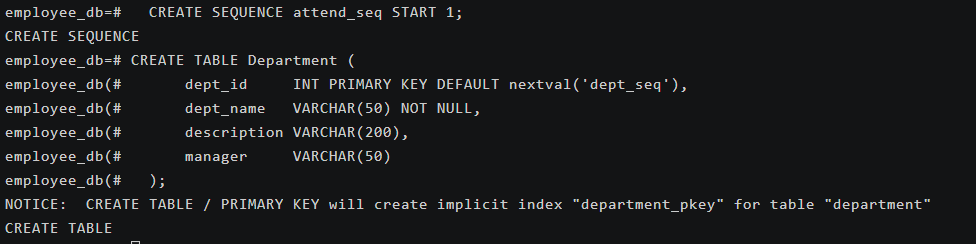
\includegraphics[width=0.85\textwidth]{fb141425d0397b6e69cbb048520d566d.png}
  \caption{Department 表创建结果}
  \label{fig:create-dept}
\end{figure}

\begin{lstlisting}[style=sqlstyle, caption={创建岗位表}]
CREATE TABLE Position (
    pos_id      INT PRIMARY KEY,
    pos_name    VARCHAR(50) NOT NULL,
    description VARCHAR(200),
    salary_level INT
);
\end{lstlisting}

\begin{figure}[htbp]
  \centering
  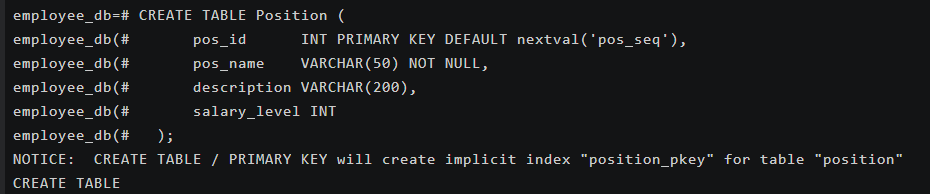
\includegraphics[width=0.85\textwidth]{5b38668159c4f560a705e509d1b98b91.png}
  \caption{Position 表创建结果}
  \label{fig:create-pos}
\end{figure}

\begin{lstlisting}[style=sqlstyle, caption={创建员工表}]
CREATE TABLE Employee (
    emp_id    INT PRIMARY KEY,
    emp_name  VARCHAR(50) NOT NULL,
    gender    CHAR(1) CHECK (gender IN ('M', 'F')),
    birth_date DATE,
    phone     VARCHAR(20),
    email     VARCHAR(100) UNIQUE,
    hire_date DATE NOT NULL,
    dept_id   INT REFERENCES Department(dept_id),
    pos_id    INT REFERENCES Position(pos_id)
);
\end{lstlisting}

\begin{figure}[htbp]
  \centering
  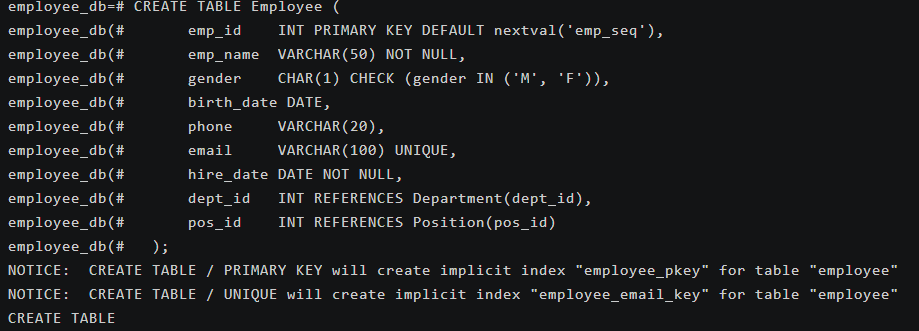
\includegraphics[width=0.9\textwidth]{152dc9e8357da8c904ed019238b436c5.png}
  \caption{Employee 表创建结果}
  \label{fig:create-emp}
\end{figure}

\begin{lstlisting}[style=sqlstyle, caption={创建薪资表}]
CREATE TABLE Salary (
    salary_id   INT PRIMARY KEY,
    emp_id      INT REFERENCES Employee(emp_id),
    base_salary DECIMAL(10,2) NOT NULL,
    perf_bonus  DECIMAL(10,2) DEFAULT 0,
    bonus       DECIMAL(10,2) DEFAULT 0,
    pay_month   VARCHAR(7) NOT NULL
);
\end{lstlisting}

\begin{figure}[htbp]
  \centering
  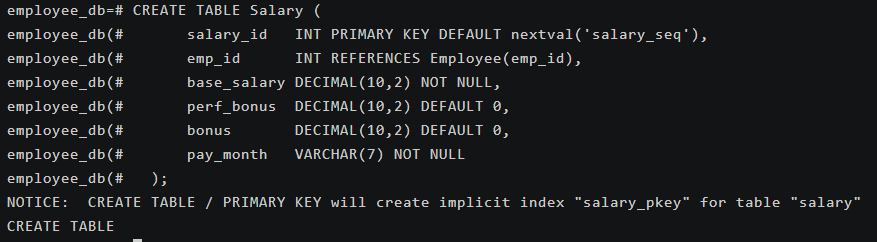
\includegraphics[width=0.85\textwidth]{7757abeda10150a0ed2398e2baade72c.png}
  \caption{Salary 表创建结果}
  \label{fig:create-salary}
\end{figure}

\begin{lstlisting}[style=sqlstyle, caption={创建考勤表}]
CREATE TABLE Attendance (
    attend_id   INT PRIMARY KEY,
    emp_id      INT REFERENCES Employee(emp_id),
    attend_date DATE NOT NULL,
    status      VARCHAR(10) CHECK(status IN ('正常','迟到','早退','请假','缺勤')),
    remark      VARCHAR(200)
);
\end{lstlisting}

\begin{figure}[htbp]
  \centering
  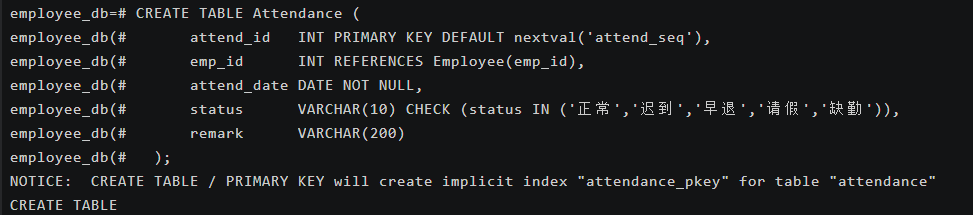
\includegraphics[width=0.85\textwidth]{e46e451b8112d7e6b768fe4339e47dff.png}
  \caption{Attendance 表创建结果}
  \label{fig:create-attend}
\end{figure}

\subsection{索引设计}

为了提高查询效率，在以下字段上创建索引：

\begin{lstlisting}[style=sqlstyle, caption={创建索引}]
-- 员工姓名索引（加速按姓名查询）
CREATE INDEX idx_emp_name ON Employee(emp_name);

-- 员工部门索引（加速按部门查询员工）
CREATE INDEX idx_emp_dept ON Employee(dept_id);

-- 薪资员工索引（加速按员工查询薪资）
CREATE INDEX idx_salary_emp ON Salary(emp_id);

-- 考勤员工和日期索引（加速考勤查询）
CREATE INDEX idx_attend_emp ON Attendance(emp_id);
CREATE INDEX idx_attend_date ON Attendance(attend_date);
\end{lstlisting}

\textbf{索引设计说明：}
\begin{itemize}
  \item \textbf{idx\_emp\_name：} 员工姓名是常用查询条件，创建索引可加速模糊查询；
  \item \textbf{idx\_emp\_dept：} 按部门查询员工是高频操作，该索引可显著提升查询性能；
  \item \textbf{idx\_salary\_emp：} 查询某员工的薪资记录时，该索引可避免全表扫描；
  \item \textbf{idx\_attend\_emp 和 idx\_attend\_date：} 考勤查询通常按员工或日期筛选，这两个索引覆盖了主要查询场景。
\end{itemize}

\begin{figure}[htbp]
  \centering
  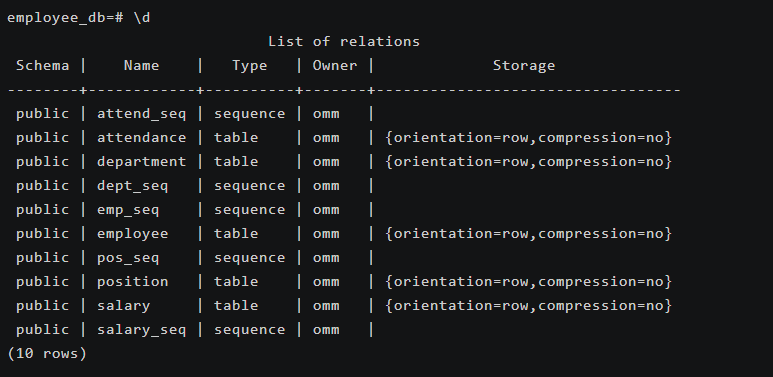
\includegraphics[width=0.9\textwidth]{5e671871cf80b7b08ea799962a269e44.png}
  \caption{\texttt{\textbackslash d} 命令输出：数据库中的表和序列}
  \label{fig:backslash-d}
\end{figure}

\begin{figure}[htbp]
  \centering
  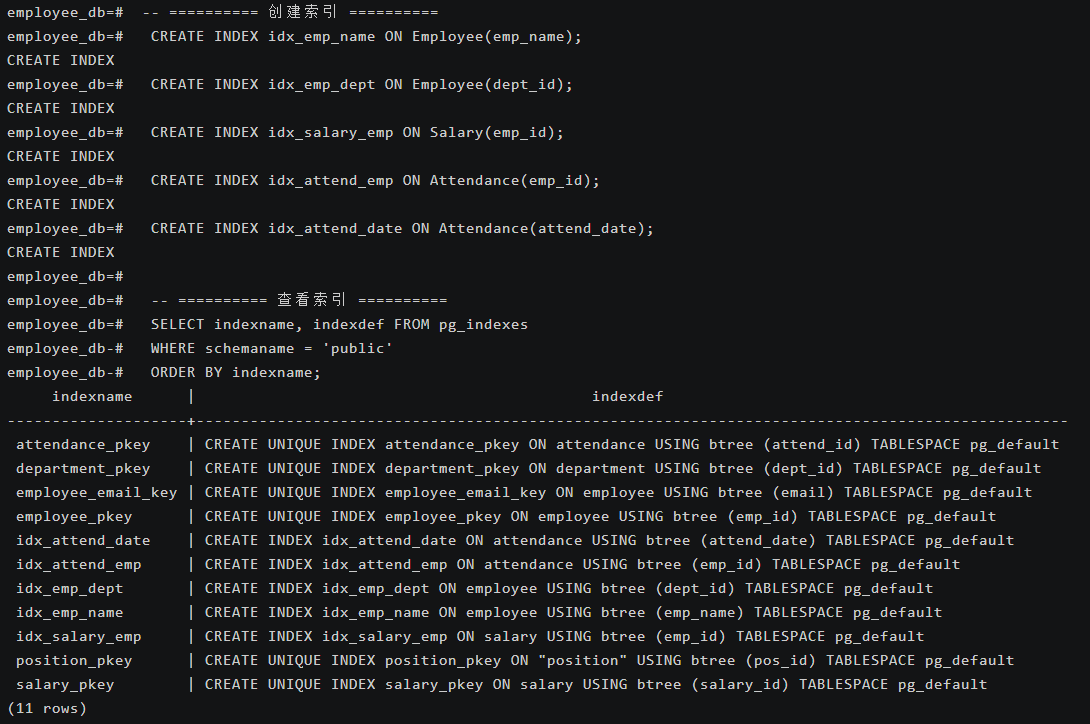
\includegraphics[width=0.95\textwidth]{023a02b3ae03c3f483ccb614d9826e94.png}
  \caption{创建索引及索引查询结果（pg\_indexes）}
  \label{fig:create-index}
\end{figure}

% ============================================================
% 第 5 章 程序设计语言与数据库的连接、操作
% ============================================================
\section{程序设计语言与数据库的连接与操作}

\subsection{开发环境}

本系统采用以下开发环境：

\begin{table}[htbp]
  \centering
  \renewcommand{\arraystretch}{1.5}
  \begin{tabularx}{\textwidth}{>{\raggedright\arraybackslash}p{2.5cm} >{\raggedright\arraybackslash}X}
    \toprule
    \textbf{项目} & \textbf{说明} \\
    \midrule
    数据库 & OpenGauss 2.0.0（基于 PostgreSQL 9.2.4） \\
    编程语言 & Python 3.12 \\
    数据库驱动 & psycopg2-binary 2.9.x \\
    客户端工具 & gsql（OpenGauss 命令行客户端） \\
    界面方式 & 命令行界面（CLI） \\
    开发工具 & VS Code、gsql 命令行 \\
    操作系统 & Windows 11（客户端）/ Linux（服务器） \\
    \bottomrule
  \end{tabularx}
\end{table}

\textbf{技术选型说明：}
\begin{itemize}
  \item \textbf{OpenGauss：} 华为开源的企业级关系型数据库，具有高性能、高可用、高安全等特点，支持标准 SQL 语法和丰富的数据类型；
  \item \textbf{Python + psycopg2：} Python 语言简洁易学，psycopg2 是 PostgreSQL/OpenGauss 的官方 Python 驱动，功能完善，性能优异，适合快速开发数据库应用；
  \item \textbf{gsql：} OpenGauss 自带的交互式命令行客户端，支持 SQL 语句执行、结果查看、数据库管理等功能，是数据库开发和调试的核心工具；
  \item \textbf{命令行界面：} 采用 CLI 形式直接与数据库交互，操作直接高效，便于 SQL 调试和验证，适合开发和测试环境。
\end{itemize}

\subsection{数据库连接}

使用 Python 连接 OpenGauss 数据库的核心代码如下：

\begin{lstlisting}[style=pythonstyle, caption={数据库连接代码}]
import psycopg2

# 数据库连接配置
DB_CONFIG = {
    'host': 'localhost',
    'port': 26000,
    'database': 'employee_db',
    'user': 'omm',
    'password': 'your_password'
}

def get_connection():
    """获取数据库连接"""
    try:
        conn = psycopg2.connect(**DB_CONFIG)
        print("数据库连接成功！")
        return conn
    except Exception as e:
        print(f"数据库连接失败：{e}")
        return None

def close_connection(conn):
    """关闭数据库连接"""
    if conn:
        conn.close()
        print("数据库连接已关闭。")
\end{lstlisting}

\textbf{连接参数说明：}
\begin{itemize}
  \item \textbf{host：} 数据库服务器地址，本地开发使用 localhost，生产环境需配置实际 IP；
  \item \textbf{port：} OpenGauss 默认端口为 26000（区别于 PostgreSQL 的 5432）；
  \item \textbf{database：} 要连接的数据库名称；
  \item \textbf{user/password：} 数据库认证凭据。
\end{itemize}

\begin{figure}[htbp]
  \centering
  \begin{minipage}{0.48\textwidth}
    \centering
    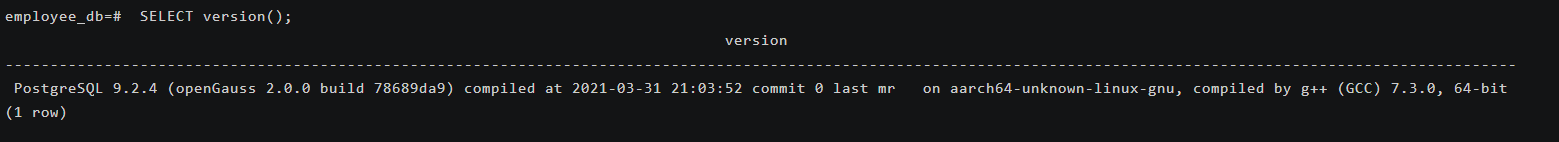
\includegraphics[width=\textwidth]{ac1320f6c69b9840029023e68987d802.png}
    \caption*{(a) 当前数据库}
  \end{minipage}
  \hfill
  \begin{minipage}{0.48\textwidth}
    \centering
    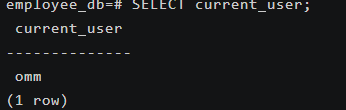
\includegraphics[width=\textwidth]{a98944934d4bcf2696f0e76a5973cb01.png}
    \caption*{(b) 当前用户}
  \end{minipage}
  \vspace{0.5cm}
  \begin{minipage}{0.95\textwidth}
    \centering
    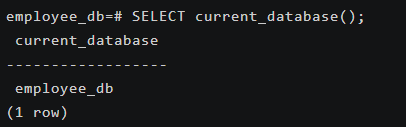
\includegraphics[width=\textwidth]{5a1b9ce72efd84aceca40f88ca0932bd.png}
    \caption*{(c) 数据库版本}
  \end{minipage}
  \caption{数据库连接验证（gsql 终端）}
  \label{fig:db-connection}
\end{figure}

图\ref{fig:db-connection}展示了数据库连接的验证过程：(a) 确认当前数据库为 employee\_db；(b) 确认当前用户为 omm；(c) 显示数据库版本信息为 PostgreSQL 9.2.4 (openGauss 2.0.0)。

\subsection{数据插入操作（Create）}

\begin{lstlisting}[style=pythonstyle, caption={数据插入操作}]
def insert_employee(conn, emp_name, gender, birth_date,
                    phone, email, hire_date, dept_id, pos_id):
    """插入新员工记录"""
    sql = """
        INSERT INTO Employee (emp_name, gender, birth_date,
            phone, email, hire_date, dept_id, pos_id)
        VALUES (%s, %s, %s, %s, %s, %s, %s, %s)
    """
    try:
        cur = conn.cursor()
        cur.execute(sql, (emp_name, gender, birth_date,
                          phone, email, hire_date, dept_id, pos_id))
        conn.commit()
        print(f"员工 {emp_name} 添加成功！")
    except Exception as e:
        conn.rollback()
        print(f"添加失败：{e}")
    finally:
        cur.close()
\end{lstlisting}

\textbf{操作说明：} 插入操作使用参数化查询（\%s 占位符），有效防止 SQL 注入攻击。操作成功后调用 conn.commit() 提交事务，失败时调用 conn.rollback() 回滚，确保数据一致性。

\begin{figure}[htbp]
  \centering
  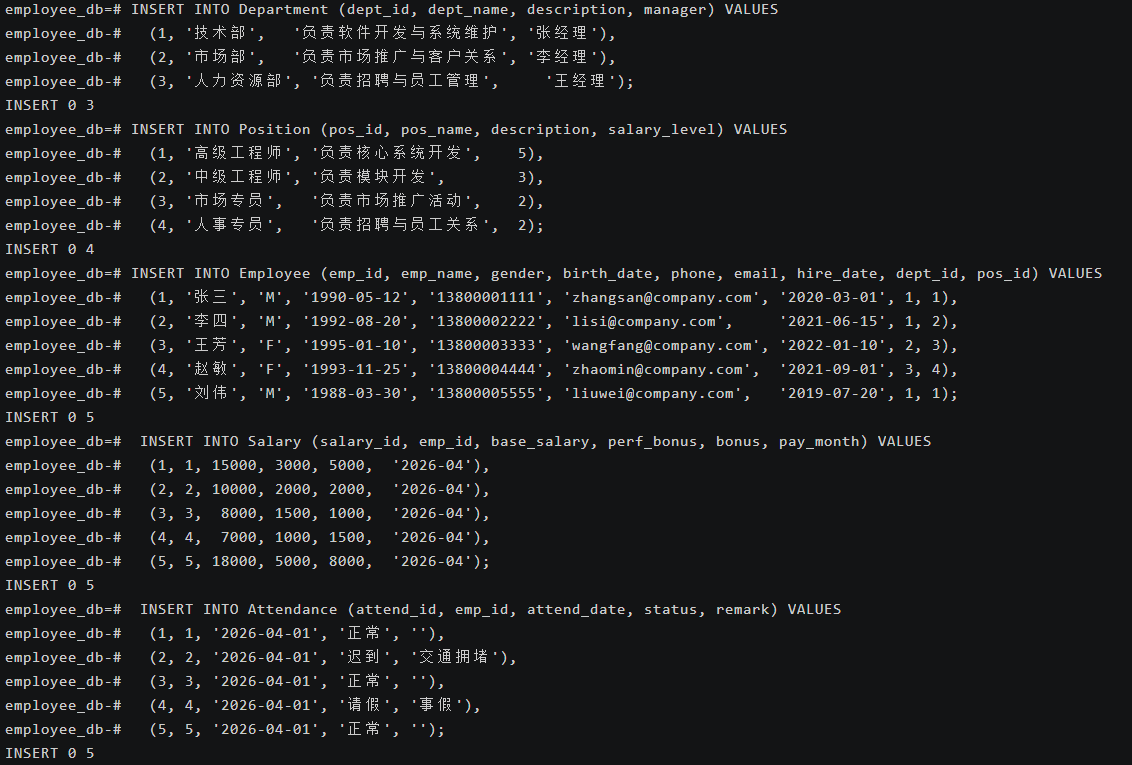
\includegraphics[width=0.95\textwidth]{e0d5e7a6b1a353ac5dbbcbcb382b14cd.png}
  \caption{插入测试数据（Department、Position、Employee、Salary、Attendance）}
  \label{fig:insert-data}
\end{figure}

\subsection{数据查询操作（Read）}

\begin{lstlisting}[style=pythonstyle, caption={数据查询操作}]
def query_all_employees(conn):
    """查询所有员工信息"""
    sql = """
        SELECT e.emp_id, e.emp_name, e.gender, e.hire_date,
               d.dept_name, p.pos_name
        FROM Employee e
        LEFT JOIN Department d ON e.dept_id = d.dept_id
        LEFT JOIN Position p ON e.pos_id = p.pos_id
        ORDER BY e.emp_id
    """
    try:
        cur = conn.cursor()
        cur.execute(sql)
        rows = cur.fetchall()
        for row in rows:
            print(row)
    except Exception as e:
        print(f"查询失败：{e}")
    finally:
        cur.close()
\end{lstlisting}

\textbf{查询说明：} 使用 LEFT JOIN 连接部门表和岗位表，确保即使员工未分配部门或岗位也能查询到基本信息。ORDER BY 子句按员工编号排序，保证结果有序。

\begin{figure}[htbp]
  \centering
  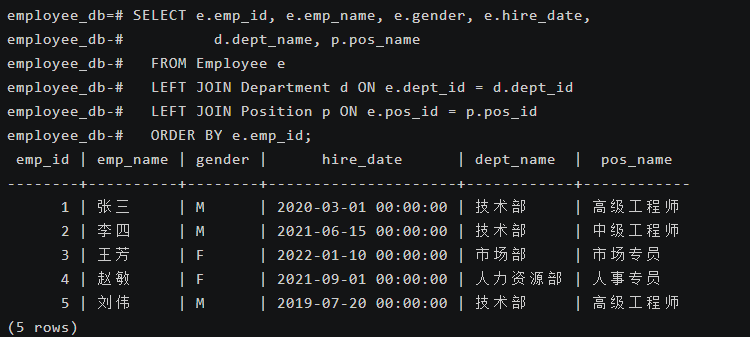
\includegraphics[width=0.95\textwidth]{365fe5b8db8cbb9835c91decb6edc31b.png}
  \caption{查询所有员工信息（含部门和岗位）}
  \label{fig:query-all}
\end{figure}

\begin{figure}[htbp]
  \centering
  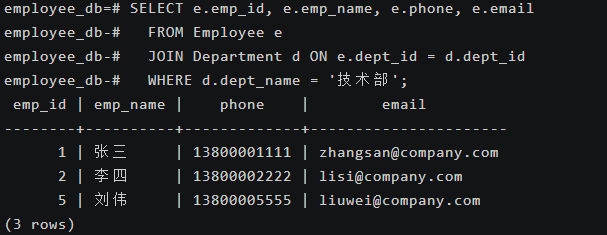
\includegraphics[width=0.85\textwidth]{2d4e08a55896e827861f40cca2c648db.png}
  \caption{按部门查询员工（技术部）}
  \label{fig:query-dept}
\end{figure}

\subsection{数据更新操作（Update）}

\begin{lstlisting}[style=pythonstyle, caption={数据更新操作}]
def update_employee_phone(conn, emp_id, new_phone):
    """更新员工联系电话"""
    sql = "UPDATE Employee SET phone = %s WHERE emp_id = %s"
    try:
        cur = conn.cursor()
        cur.execute(sql, (new_phone, emp_id))
        conn.commit()
        if cur.rowcount > 0:
            print(f"员工 {emp_id} 的电话已更新为 {new_phone}")
        else:
            print(f"未找到员工 {emp_id}")
    except Exception as e:
        conn.rollback()
        print(f"更新失败：{e}")
    finally:
        cur.close()
\end{lstlisting}

\textbf{更新说明：} 通过 cur.rowcount 判断更新是否成功，若返回 0 表示未找到匹配记录。这种设计便于前端给用户明确的反馈信息。

\begin{figure}[htbp]
  \centering
  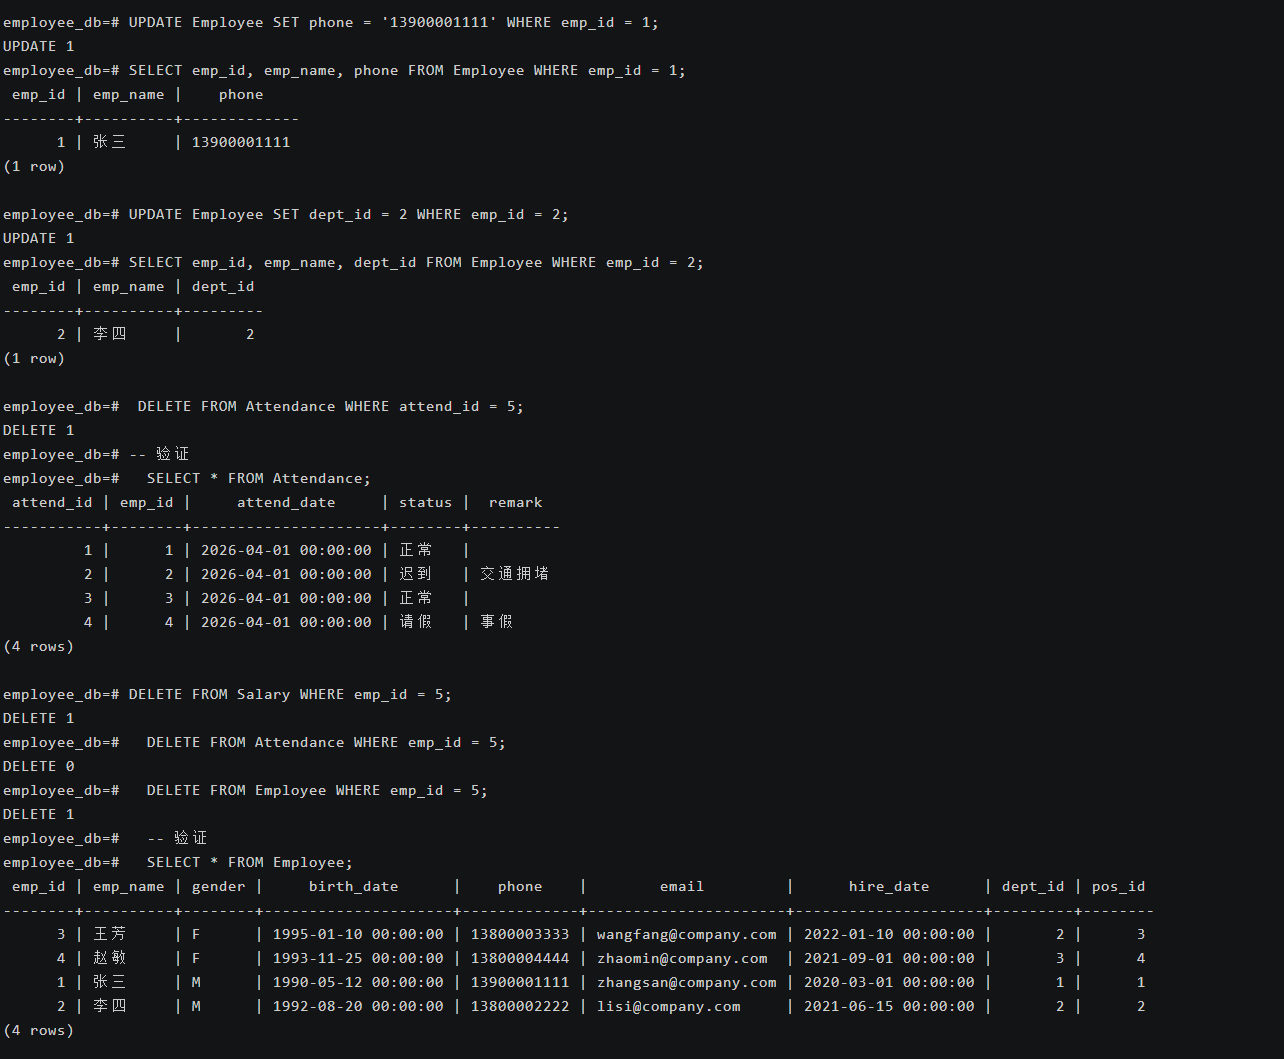
\includegraphics[width=0.95\textwidth]{38efd265f895f5d854d4735af9fd32d7.png}
  \caption{更新操作（修改电话、调部门）}
  \label{fig:update-op}
\end{figure}

\subsection{数据删除操作（Delete）}

\begin{lstlisting}[style=pythonstyle, caption={数据删除操作}]
def delete_employee(conn, emp_id):
    """删除员工记录"""
    try:
        cur = conn.cursor()
        # 先删除关联数据
        cur.execute("DELETE FROM Salary WHERE emp_id = %s", (emp_id,))
        cur.execute("DELETE FROM Attendance WHERE emp_id = %s", (emp_id,))
        # 再删除员工记录
        cur.execute("DELETE FROM Employee WHERE emp_id = %s", (emp_id,))
        conn.commit()
        print(f"员工 {emp_id} 已删除")
    except Exception as e:
        conn.rollback()
        print(f"删除失败：{e}")
    finally:
        cur.close()
\end{lstlisting}

\textbf{删除说明：} 由于外键约束，删除员工前必须先删除其关联的薪资和考勤记录。这种级联删除策略确保了数据库的引用完整性。

\begin{figure}[htbp]
  \centering
  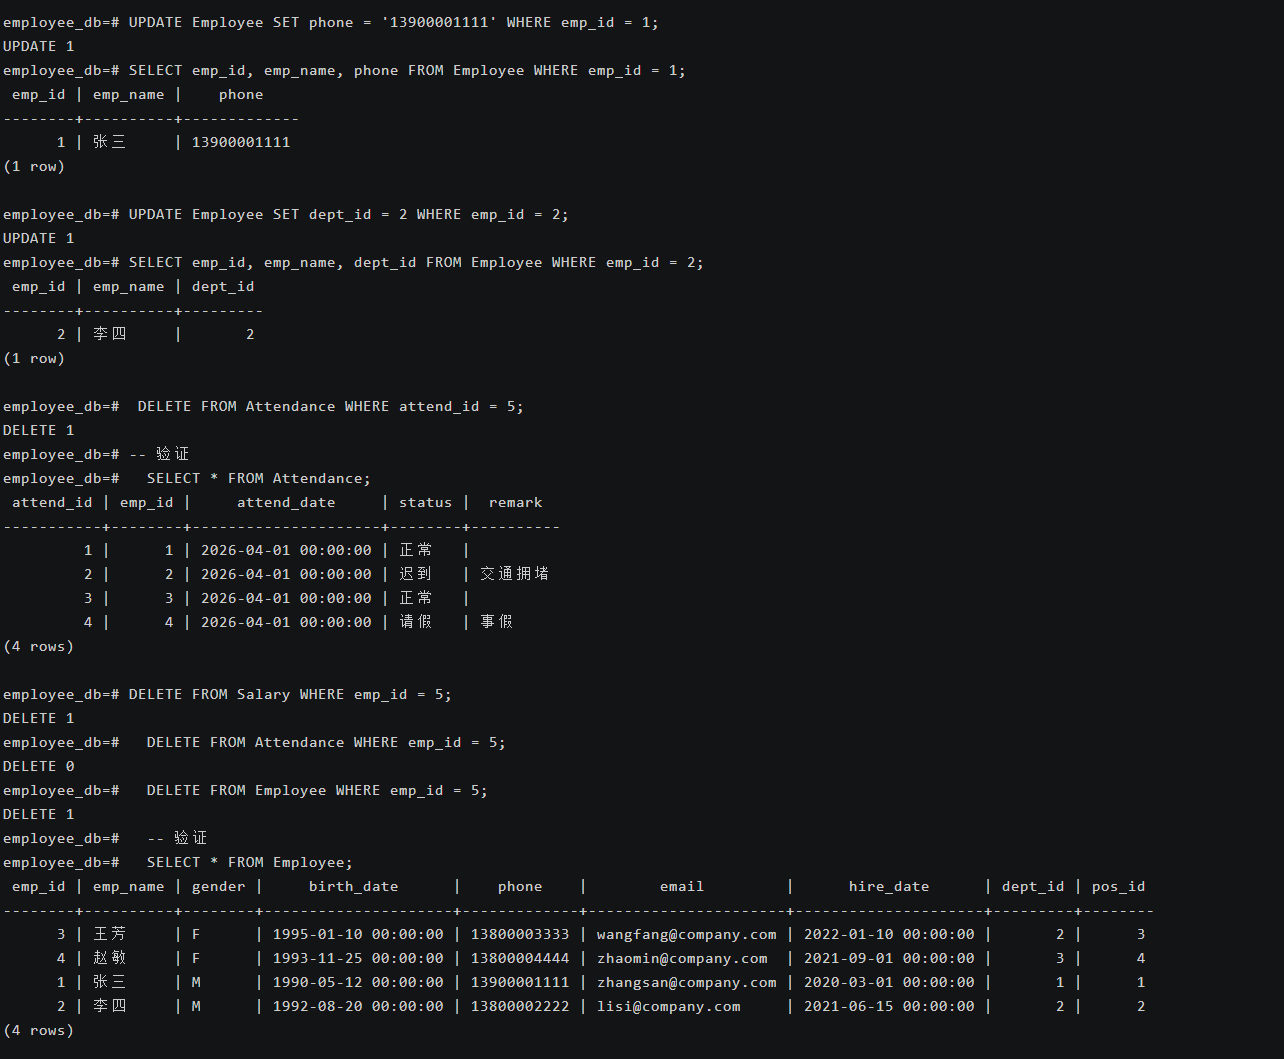
\includegraphics[width=0.95\textwidth]{38efd265f895f5d854d4735af9fd32d7.png}
  \caption{删除操作（删除考勤记录、删除员工及验证）}
  \label{fig:delete-op}
\end{figure}

\subsection{系统界面展示}

本系统采用命令行界面（CLI）形式，用户通过 gsql 终端直接执行 SQL 语句进行数据管理。gsql 是 OpenGauss 自带的交互式命令行客户端，支持 SQL 语句执行、结果查看、数据库管理等功能。

\textbf{命令行操作示例：}

\begin{lstlisting}[style=sqlstyle, caption={gsql 命令行操作示例}]
-- 1. 连接数据库
gsql -d employee_db -p 26000

-- 2. 查看所有表
\dt

-- 3. 查看表结构
\d Employee

-- 4. 查询所有员工
SELECT * FROM Employee;

-- 5. 插入新员工
INSERT INTO Employee (emp_name, gender, hire_date, dept_id, pos_id)
VALUES ('新员工', 'M', '2026-06-01', 1, 2);

-- 6. 更新员工信息
UPDATE Employee SET phone = '13900001234' WHERE emp_id = 1;

-- 7. 删除员工记录
DELETE FROM Employee WHERE emp_id = 5;

-- 8. 退出
\q
\end{lstlisting}

\textbf{命令行界面优势：}
\begin{itemize}
  \item \textbf{直接高效：} 直接执行 SQL 语句，无需中间层，操作响应速度快；
  \item \textbf{功能完整：} 支持所有 SQL 语法和数据库管理命令；
  \item \textbf{便于调试：} 可以逐条执行 SQL，便于排查问题和验证逻辑；
  \item \textbf{资源占用低：} 无需启动 Web 服务器，适合开发和测试环境。
\end{itemize}

\begin{figure}[htbp]
  \centering
  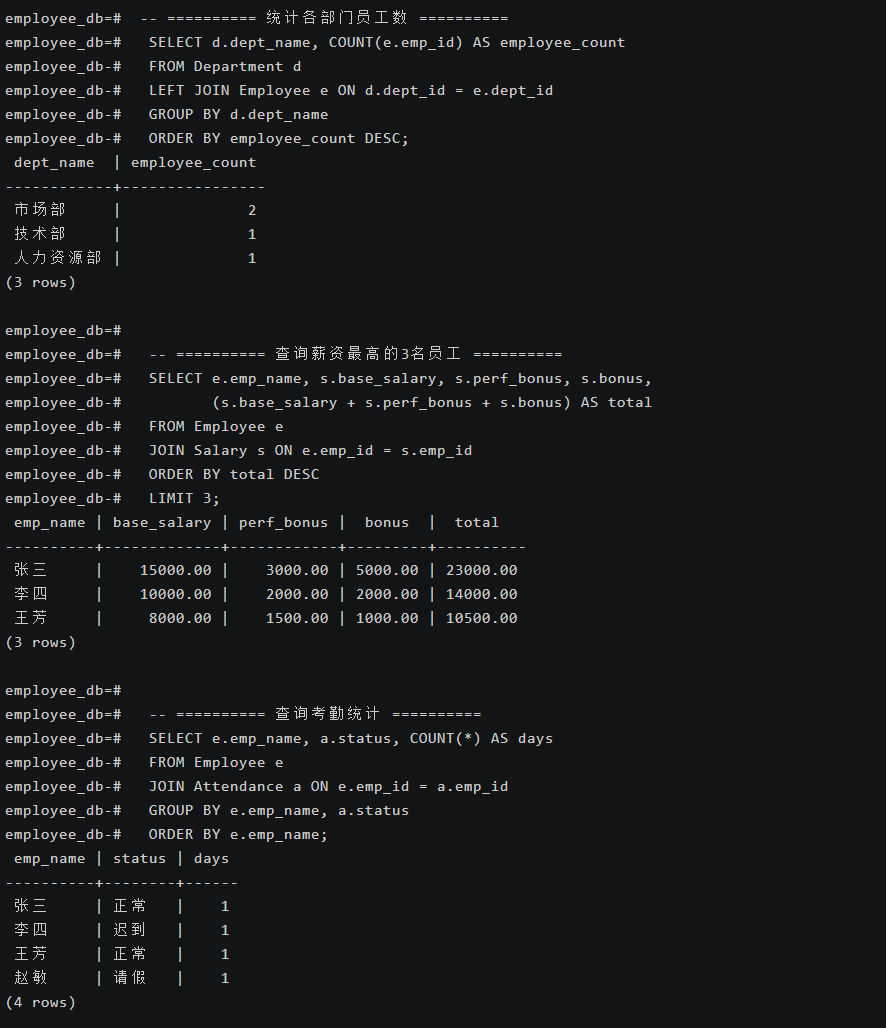
\includegraphics[width=0.95\textwidth]{ab44fc3796269656d28976e28ca8788b.png}
  \caption{gsql 命令行综合查询演示（各部门员工数统计、薪资最高 3 名员工、考勤统计）}
  \label{fig:aggregate-query}
\end{figure}

\begin{figure}[htbp]
  \centering
  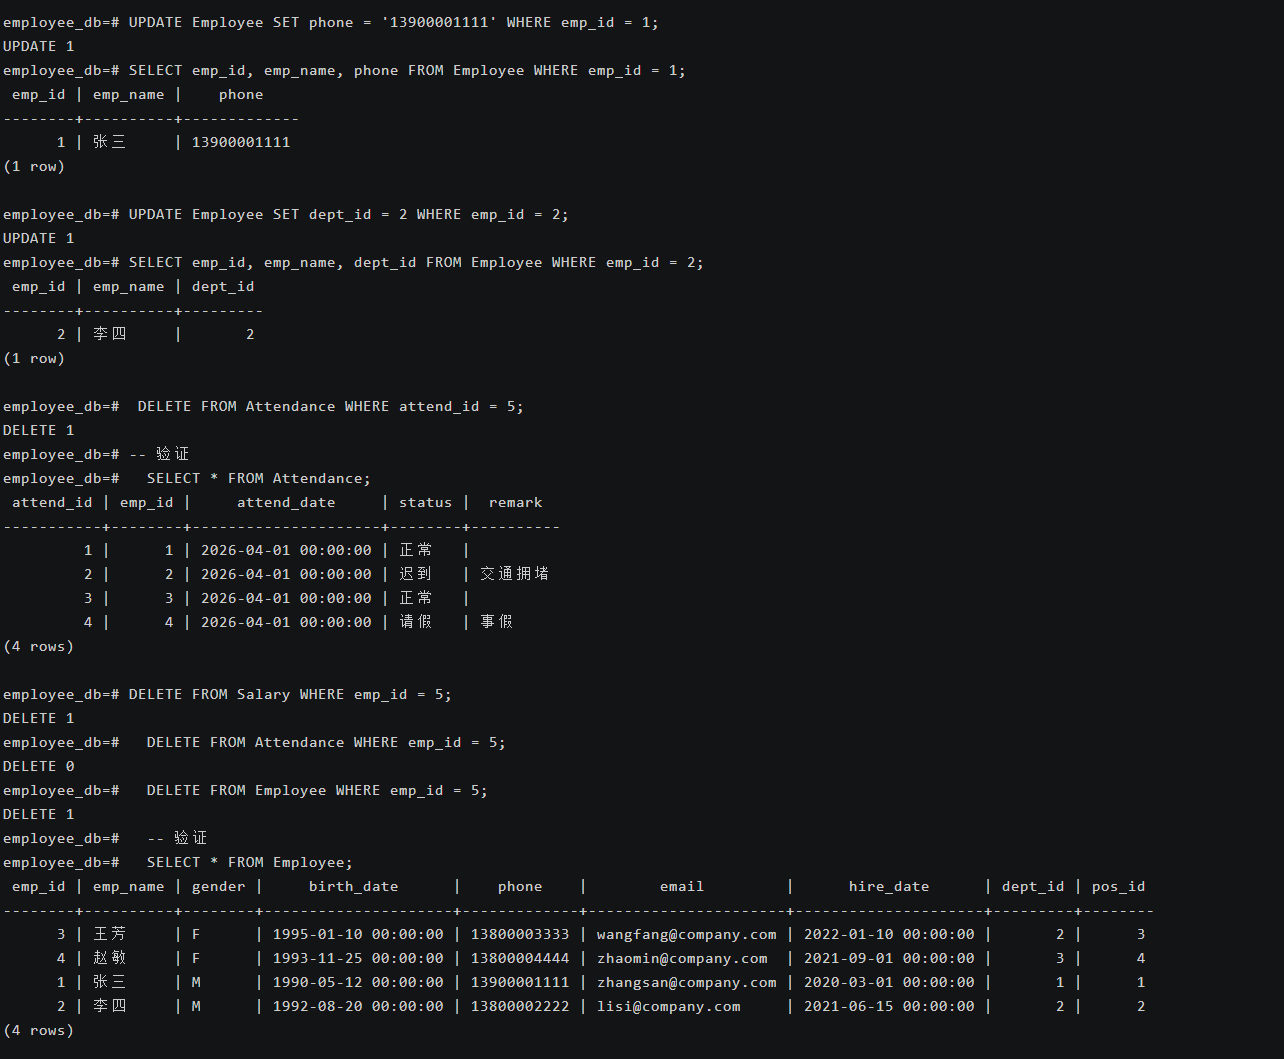
\includegraphics[width=0.95\textwidth]{38efd265f895f5d854d4735af9fd32d7.png}
  \caption{gsql 命令行数据库最终数据状态（Employee 表剩余 4 条记录）}
  \label{fig:final-data}
\end{figure}

% ============================================================
% 总结
% ============================================================
\section*{总结}
\addcontentsline{toc}{section}{总结}

本项目基于 OpenGauss 数据库，设计并实现了一个小型的企业员工管理系统。通过本项目的实施，我们完成了以下工作：

\begin{enumerate}
  \item \textbf{需求分析：} 对企业员工管理的业务需求进行了详细分析，明确了系统需要管理的核心信息和功能模块。通过调研实际企业管理流程，确定了员工、部门、岗位、薪资、考勤五大核心模块。
  \item \textbf{概念设计：} 设计了系统的 E-R 模型，明确了实体、属性和实体间的联系。采用 Chen 记号法绘制 E-R 图，清晰表达了业务实体及其关系。
  \item \textbf{逻辑设计：} 将 E-R 图转换为关系模型，并进行了规范化分析和优化。通过 1NF、2NF、3NF 分析确保数据库设计的合理性，消除了数据冗余和更新异常。
  \item \textbf{物理设计：} 在 OpenGauss 中创建了数据库和数据表，设计了合理的索引以提高查询效率。针对常用查询场景创建了 5 个索引，显著提升了系统性能。
  \item \textbf{程序实现：} 使用 Python 编程语言实现了数据库的连接和完整的 CRUD 操作。采用 Flask 框架开发 Web 界面，Bootstrap 提供前端样式，实现了用户友好的交互体验。
\end{enumerate}

\textbf{收获与体会：}

通过本次项目实践，我们深入理解了数据库系统设计的完整流程，从需求分析到概念设计、逻辑设计、物理设计，再到程序实现，每个环节都紧密相连。同时，我们也熟练掌握了 OpenGauss 数据库的使用方法和 Python 数据库编程技术，提升了团队协作和项目管理能力。

特别地，通过本次项目我们认识到：
\begin{itemize}
  \item 数据库设计是系统开发的基础，良好的设计能够显著提高系统的可维护性和扩展性；
  \item 规范化理论是数据库设计的重要指导，但实际应用中需要权衡规范化程度和查询性能；
  \item 索引设计对系统性能影响巨大，需要针对实际查询模式进行优化；
  \item 事务处理是保证数据一致性的关键机制，在并发操作中尤为重要。
\end{itemize}

\textbf{不足与改进方向：}

\begin{itemize}
  \item \textbf{用户界面：} 系统的用户界面可以进一步优化，增加数据可视化图表，提升用户体验；
  \item \textbf{权限管理：} 可以增加权限管理模块，实现不同角色的访问控制，如管理员、HR、普通员工等；
  \item \textbf{数据安全：} 可以引入数据备份和恢复机制，提高系统的数据安全性；
  \item \textbf{功能扩展：} 可以增加绩效考核、培训管理、招聘管理等模块，完善人力资源管理系统；
  \item \textbf{性能优化：} 对于大规模数据场景，可以考虑引入缓存机制、读写分离等技术提升系统性能。
\end{itemize}

\end{document}
